% Options for packages loaded elsewhere
\PassOptionsToPackage{unicode}{hyperref}
\PassOptionsToPackage{hyphens}{url}
%
\documentclass[
  english,
  man, fleqn, noextraspace]{apa6}
\usepackage{lmodern}
\usepackage{amssymb,amsmath}
\usepackage{ifxetex,ifluatex}
\ifnum 0\ifxetex 1\fi\ifluatex 1\fi=0 % if pdftex
  \usepackage[T1]{fontenc}
  \usepackage[utf8]{inputenc}
  \usepackage{textcomp} % provide euro and other symbols
\else % if luatex or xetex
  \usepackage{unicode-math}
  \defaultfontfeatures{Scale=MatchLowercase}
  \defaultfontfeatures[\rmfamily]{Ligatures=TeX,Scale=1}
\fi
% Use upquote if available, for straight quotes in verbatim environments
\IfFileExists{upquote.sty}{\usepackage{upquote}}{}
\IfFileExists{microtype.sty}{% use microtype if available
  \usepackage[]{microtype}
  \UseMicrotypeSet[protrusion]{basicmath} % disable protrusion for tt fonts
}{}
\makeatletter
\@ifundefined{KOMAClassName}{% if non-KOMA class
  \IfFileExists{parskip.sty}{%
    \usepackage{parskip}
  }{% else
    \setlength{\parindent}{0pt}
    \setlength{\parskip}{6pt plus 2pt minus 1pt}}
}{% if KOMA class
  \KOMAoptions{parskip=half}}
\makeatother
\usepackage{xcolor}
\IfFileExists{xurl.sty}{\usepackage{xurl}}{} % add URL line breaks if available
\IfFileExists{bookmark.sty}{\usepackage{bookmark}}{\usepackage{hyperref}}
\hypersetup{
  pdftitle={EDLD 651 Final Project Draft},
  pdfauthor={Anwesha Guha1, Heidi Iwashita1, Christopher Loan1, Adam Nielsen1, \& Aaron Rothbart1},
  pdflang={en-EN},
  pdfkeywords={keywords},
  hidelinks,
  pdfcreator={LaTeX via pandoc}}
\urlstyle{same} % disable monospaced font for URLs
\usepackage{color}
\usepackage{fancyvrb}
\newcommand{\VerbBar}{|}
\newcommand{\VERB}{\Verb[commandchars=\\\{\}]}
\DefineVerbatimEnvironment{Highlighting}{Verbatim}{commandchars=\\\{\}}
% Add ',fontsize=\small' for more characters per line
\usepackage{framed}
\definecolor{shadecolor}{RGB}{248,248,248}
\newenvironment{Shaded}{\begin{snugshade}}{\end{snugshade}}
\newcommand{\AlertTok}[1]{\textcolor[rgb]{0.94,0.16,0.16}{#1}}
\newcommand{\AnnotationTok}[1]{\textcolor[rgb]{0.56,0.35,0.01}{\textbf{\textit{#1}}}}
\newcommand{\AttributeTok}[1]{\textcolor[rgb]{0.77,0.63,0.00}{#1}}
\newcommand{\BaseNTok}[1]{\textcolor[rgb]{0.00,0.00,0.81}{#1}}
\newcommand{\BuiltInTok}[1]{#1}
\newcommand{\CharTok}[1]{\textcolor[rgb]{0.31,0.60,0.02}{#1}}
\newcommand{\CommentTok}[1]{\textcolor[rgb]{0.56,0.35,0.01}{\textit{#1}}}
\newcommand{\CommentVarTok}[1]{\textcolor[rgb]{0.56,0.35,0.01}{\textbf{\textit{#1}}}}
\newcommand{\ConstantTok}[1]{\textcolor[rgb]{0.00,0.00,0.00}{#1}}
\newcommand{\ControlFlowTok}[1]{\textcolor[rgb]{0.13,0.29,0.53}{\textbf{#1}}}
\newcommand{\DataTypeTok}[1]{\textcolor[rgb]{0.13,0.29,0.53}{#1}}
\newcommand{\DecValTok}[1]{\textcolor[rgb]{0.00,0.00,0.81}{#1}}
\newcommand{\DocumentationTok}[1]{\textcolor[rgb]{0.56,0.35,0.01}{\textbf{\textit{#1}}}}
\newcommand{\ErrorTok}[1]{\textcolor[rgb]{0.64,0.00,0.00}{\textbf{#1}}}
\newcommand{\ExtensionTok}[1]{#1}
\newcommand{\FloatTok}[1]{\textcolor[rgb]{0.00,0.00,0.81}{#1}}
\newcommand{\FunctionTok}[1]{\textcolor[rgb]{0.00,0.00,0.00}{#1}}
\newcommand{\ImportTok}[1]{#1}
\newcommand{\InformationTok}[1]{\textcolor[rgb]{0.56,0.35,0.01}{\textbf{\textit{#1}}}}
\newcommand{\KeywordTok}[1]{\textcolor[rgb]{0.13,0.29,0.53}{\textbf{#1}}}
\newcommand{\NormalTok}[1]{#1}
\newcommand{\OperatorTok}[1]{\textcolor[rgb]{0.81,0.36,0.00}{\textbf{#1}}}
\newcommand{\OtherTok}[1]{\textcolor[rgb]{0.56,0.35,0.01}{#1}}
\newcommand{\PreprocessorTok}[1]{\textcolor[rgb]{0.56,0.35,0.01}{\textit{#1}}}
\newcommand{\RegionMarkerTok}[1]{#1}
\newcommand{\SpecialCharTok}[1]{\textcolor[rgb]{0.00,0.00,0.00}{#1}}
\newcommand{\SpecialStringTok}[1]{\textcolor[rgb]{0.31,0.60,0.02}{#1}}
\newcommand{\StringTok}[1]{\textcolor[rgb]{0.31,0.60,0.02}{#1}}
\newcommand{\VariableTok}[1]{\textcolor[rgb]{0.00,0.00,0.00}{#1}}
\newcommand{\VerbatimStringTok}[1]{\textcolor[rgb]{0.31,0.60,0.02}{#1}}
\newcommand{\WarningTok}[1]{\textcolor[rgb]{0.56,0.35,0.01}{\textbf{\textit{#1}}}}
\usepackage{graphicx,grffile}
\makeatletter
\def\maxwidth{\ifdim\Gin@nat@width>\linewidth\linewidth\else\Gin@nat@width\fi}
\def\maxheight{\ifdim\Gin@nat@height>\textheight\textheight\else\Gin@nat@height\fi}
\makeatother
% Scale images if necessary, so that they will not overflow the page
% margins by default, and it is still possible to overwrite the defaults
% using explicit options in \includegraphics[width, height, ...]{}
\setkeys{Gin}{width=\maxwidth,height=\maxheight,keepaspectratio}
% Set default figure placement to htbp
\makeatletter
\def\fps@figure{htbp}
\makeatother
\setlength{\emergencystretch}{3em} % prevent overfull lines
\providecommand{\tightlist}{%
  \setlength{\itemsep}{0pt}\setlength{\parskip}{0pt}}
\setcounter{secnumdepth}{-\maxdimen} % remove section numbering
% Make \paragraph and \subparagraph free-standing
\ifx\paragraph\undefined\else
  \let\oldparagraph\paragraph
  \renewcommand{\paragraph}[1]{\oldparagraph{#1}\mbox{}}
\fi
\ifx\subparagraph\undefined\else
  \let\oldsubparagraph\subparagraph
  \renewcommand{\subparagraph}[1]{\oldsubparagraph{#1}\mbox{}}
\fi
% Manuscript styling
\usepackage{upgreek}
\captionsetup{font=singlespacing,justification=justified}

% Table formatting
\usepackage{longtable}
\usepackage{lscape}
% \usepackage[counterclockwise]{rotating}   % Landscape page setup for large tables
\usepackage{multirow}		% Table styling
\usepackage{tabularx}		% Control Column width
\usepackage[flushleft]{threeparttable}	% Allows for three part tables with a specified notes section
\usepackage{threeparttablex}            % Lets threeparttable work with longtable

% Create new environments so endfloat can handle them
% \newenvironment{ltable}
%   {\begin{landscape}\begin{center}\begin{threeparttable}}
%   {\end{threeparttable}\end{center}\end{landscape}}
\newenvironment{lltable}{\begin{landscape}\begin{center}\begin{ThreePartTable}}{\end{ThreePartTable}\end{center}\end{landscape}}

% Enables adjusting longtable caption width to table width
% Solution found at http://golatex.de/longtable-mit-caption-so-breit-wie-die-tabelle-t15767.html
\makeatletter
\newcommand\LastLTentrywidth{1em}
\newlength\longtablewidth
\setlength{\longtablewidth}{1in}
\newcommand{\getlongtablewidth}{\begingroup \ifcsname LT@\roman{LT@tables}\endcsname \global\longtablewidth=0pt \renewcommand{\LT@entry}[2]{\global\advance\longtablewidth by ##2\relax\gdef\LastLTentrywidth{##2}}\@nameuse{LT@\roman{LT@tables}} \fi \endgroup}

% \setlength{\parindent}{0.5in}
% \setlength{\parskip}{0pt plus 0pt minus 0pt}

% \usepackage{etoolbox}
\makeatletter
\patchcmd{\HyOrg@maketitle}
  {\section{\normalfont\normalsize\abstractname}}
  {\section*{\normalfont\normalsize\abstractname}}
  {}{\typeout{Failed to patch abstract.}}
\patchcmd{\HyOrg@maketitle}
  {\section{\protect\normalfont{\@title}}}
  {\section*{\protect\normalfont{\@title}}}
  {}{\typeout{Failed to patch title.}}
\makeatother
\shorttitle{Final\_Draft}
\keywords{keywords\newline\indent Word count: X}
\DeclareDelayedFloatFlavor{ThreePartTable}{table}
\DeclareDelayedFloatFlavor{lltable}{table}
\DeclareDelayedFloatFlavor*{longtable}{table}
\makeatletter
\renewcommand{\efloat@iwrite}[1]{\immediate\expandafter\protected@write\csname efloat@post#1\endcsname{}}
\makeatother
\usepackage{lineno}

\linenumbers
\usepackage{csquotes}
\raggedbottom
\setlength{\parskip}{0pt}
\ifxetex
  % Load polyglossia as late as possible: uses bidi with RTL langages (e.g. Hebrew, Arabic)
  \usepackage{polyglossia}
  \setmainlanguage[]{english}
\else
  \usepackage[shorthands=off,main=english]{babel}
\fi

\title{EDLD 651 Final Project Draft}
\author{Anwesha Guha\textsuperscript{1}, Heidi Iwashita\textsuperscript{1}, Christopher Loan\textsuperscript{1}, Adam Nielsen\textsuperscript{1}, \& Aaron Rothbart\textsuperscript{1}}
\date{}


\authornote{

All work done herein represents contributions from all authors equally. Author order is alphabetical.

}

\affiliation{\vspace{0.5cm}\textsuperscript{1} University of Oregon}

\abstract{
FILL IN ABSTRACT IF WANTED
}



\begin{document}
\maketitle

\hypertarget{introduction}{%
\section{Introduction}\label{introduction}}

We explore proportion of graduation (outcome), across several categorical variables. In particular, we plan to focus on comparisons of two groups who have historically had unequal access to resources: English language learners (ELL) vs.~English proficient (EP) students \& Special Education (SPED) status vs.~non-SPED status.

Not only will we report these outcomes across different groups, we will also explore these across boroughs, too, to see if these groups are succeeding equally across boroughs----as measured by graduation outcomes----compared to the English proficient students in their boroughs.

\hypertarget{methods}{%
\section{Methods}\label{methods}}

We retrieved the data collected by the Department of Education from

Information about variables, how they were measured here

Information about regents examinations here

\hypertarget{participants}{%
\subsection{Participants}\label{participants}}

Explain participants' from what we have in data.

First, we import and clean our data:

\begin{Shaded}
\begin{Highlighting}[]
\NormalTok{raw_grad <-}\StringTok{ }\KeywordTok{import}\NormalTok{(}\KeywordTok{here}\NormalTok{(}\StringTok{"data"}\NormalTok{, }\StringTok{"2005-2010__Graduation_Outcomes_-__By_Borough.csv"}\NormalTok{))}
\NormalTok{grad <-}\StringTok{ }\NormalTok{raw_grad }\OperatorTok\StringTok{ }
\StringTok{  }\KeywordTok{clean_names}\NormalTok{() }\OperatorTok\StringTok{ }
\StringTok{  }\KeywordTok{as_tibble}\NormalTok{()}

\KeywordTok{summary}\NormalTok{(grad}\OperatorTok{$}\NormalTok{cohort) }\CommentTok{# we see here that 'Aug 2006' needs to be changed to '2006' for consistency}
\end{Highlighting}
\end{Shaded}

\begin{verbatim}
##    Length     Class      Mode 
##       385 character character
\end{verbatim}

\begin{Shaded}
\begin{Highlighting}[]
\NormalTok{grad}\OperatorTok{$}\NormalTok{cohort <-}\StringTok{  }\KeywordTok{as.numeric}\NormalTok{(}\KeywordTok{sub}\NormalTok{(}\StringTok{"Aug 2006"}\NormalTok{, }\StringTok{"2006"}\NormalTok{, grad}\OperatorTok{$}\NormalTok{cohort))}

\KeywordTok{head}\NormalTok{(grad)}\CommentTok{#need to change var names to make legible, perhaps subset data to only include the variables we are interested in and want to display}
\end{Highlighting}
\end{Shaded}

\begin{verbatim}
## # A tibble: 6 x 22
##   demographic borough cohort total_cohort total_grads_n total_grads_per~
##   <chr>       <chr>    <dbl>        <int>         <int>            <dbl>
## 1 Borough To~ Bronx     2001        11453          4913             42.9
## 2 Borough To~ Bronx     2002        12032          5328             44.3
## 3 Borough To~ Bronx     2003        13632          6389             46.9
## 4 Borough To~ Bronx     2004        14364          7448             51.9
## 5 Borough To~ Bronx     2005        15175          8229             54.2
## 6 Borough To~ Bronx     2006        15579          8524             54.7
## # ... with 16 more variables: total_regents_n <int>,
## #   total_regents_percent_of_cohort <dbl>,
## #   total_regents_percent_of_grads <dbl>, advanced_regents_n <int>,
## #   advanced_regents_percent_of_cohort <dbl>,
## #   advanced_regents_percent_of_grads <dbl>, regents_w_o_advanced_n <int>,
## #   regents_w_o_advanced_percent_of_cohort <dbl>,
## #   regents_w_o_advanced_percent_of_grads <dbl>, local_n <int>,
## #   local_percent_of_cohort <dbl>, local_percent_of_grads <dbl>,
## #   still_enrolled_n <int>, still_enrolled_percent_of_cohort <dbl>,
## #   dropped_out_n <int>, dropped_out_percent_of_cohort <dbl>
\end{verbatim}

\begin{Shaded}
\begin{Highlighting}[]
\CommentTok{# Do we want to use recode() or rename()? Also, does it make more sense to leave all of the columns until we get to the 'select' r-chunk? -Adam}
\end{Highlighting}
\end{Shaded}

\hypertarget{pivots}{%
\subsection{PIVOTS}\label{pivots}}

The data we are starting with are already tidy, but for the purposes of demonstrating our rather acute proficiency in our \emph{ability} to tidy data, in this segment will make the data untidy and then tidy it once more.

\begin{Shaded}
\begin{Highlighting}[]
\NormalTok{messy_grad <-}\StringTok{ }\NormalTok{grad }\OperatorTok\StringTok{ }
\StringTok{  }\KeywordTok{pivot_wider}\NormalTok{(}\DataTypeTok{names_from =}\NormalTok{ borough,}
              \DataTypeTok{values_from =}\NormalTok{ total_cohort)}
\KeywordTok{head}\NormalTok{(messy_grad)}
\end{Highlighting}
\end{Shaded}

\begin{verbatim}
## # A tibble: 6 x 25
##   demographic cohort total_grads_n total_grads_per~ total_regents_n
##   <chr>        <dbl>         <int>            <dbl>           <int>
## 1 Borough To~   2001          4913             42.9            2644
## 2 Borough To~   2002          5328             44.3            3118
## 3 Borough To~   2003          6389             46.9            3861
## 4 Borough To~   2004          7448             51.9            4625
## 5 Borough To~   2005          8229             54.2            5618
## 6 Borough To~   2006          8524             54.7            6312
## # ... with 20 more variables: total_regents_percent_of_cohort <dbl>,
## #   total_regents_percent_of_grads <dbl>, advanced_regents_n <int>,
## #   advanced_regents_percent_of_cohort <dbl>,
## #   advanced_regents_percent_of_grads <dbl>, regents_w_o_advanced_n <int>,
## #   regents_w_o_advanced_percent_of_cohort <dbl>,
## #   regents_w_o_advanced_percent_of_grads <dbl>, local_n <int>,
## #   local_percent_of_cohort <dbl>, local_percent_of_grads <dbl>,
## #   still_enrolled_n <int>, still_enrolled_percent_of_cohort <dbl>,
## #   dropped_out_n <int>, dropped_out_percent_of_cohort <dbl>, Bronx <int>,
## #   Brooklyn <int>, Manhattan <int>, Queens <int>, `Staten Island` <int>
\end{verbatim}

\begin{Shaded}
\begin{Highlighting}[]
\NormalTok{clean_grad <-}\StringTok{ }\NormalTok{messy_grad }\OperatorTok\StringTok{ }
\StringTok{  }\KeywordTok{pivot_longer}\NormalTok{(}\DataTypeTok{cols =} \KeywordTok{c}\NormalTok{(}\StringTok{"Bronx"}\OperatorTok{:}\StringTok{"Staten Island"}\NormalTok{),}
               \DataTypeTok{names_to =} \StringTok{"borough"}\NormalTok{,}
               \DataTypeTok{values_to =} \StringTok{"total_cohort"}\NormalTok{,}
               \DataTypeTok{values_drop_na =} \OtherTok{TRUE}\NormalTok{)}

\NormalTok{clean_grad <-}\StringTok{ }\NormalTok{clean_grad[, }\KeywordTok{c}\NormalTok{(}\DecValTok{1}\NormalTok{,}\DecValTok{21}\NormalTok{,}\DecValTok{2}\NormalTok{,}\DecValTok{22}\NormalTok{,}\DecValTok{3}\OperatorTok{:}\DecValTok{20}\NormalTok{)]}
\KeywordTok{kable}\NormalTok{(clean_grad)}
\end{Highlighting}
\end{Shaded}

\begin{tabular}{l|l|r|r|r|r|r|r|r|r|r|r|r|r|r|r|r|r|r|r|r|r}
\hline
demographic & borough & cohort & total\_cohort & total\_grads\_n & total\_grads\_percent\_of\_cohort & total\_regents\_n & total\_regents\_percent\_of\_cohort & total\_regents\_percent\_of\_grads & advanced\_regents\_n & advanced\_regents\_percent\_of\_cohort & advanced\_regents\_percent\_of\_grads & regents\_w\_o\_advanced\_n & regents\_w\_o\_advanced\_percent\_of\_cohort & regents\_w\_o\_advanced\_percent\_of\_grads & local\_n & local\_percent\_of\_cohort & local\_percent\_of\_grads & still\_enrolled\_n & still\_enrolled\_percent\_of\_cohort & dropped\_out\_n & dropped\_out\_percent\_of\_cohort\\
\hline
Borough Total & Bronx & 2001 & 11453 & 4913 & 42.9 & 2644 & 23.1 & 53.8 & 998 & 8.7 & 20.3 & 1646 & 14.4 & 33.5 & 2271 & 19.8 & 46.2 & 3512 & 30.7 & 2438 & 21.3\\
\hline
Borough Total & Bronx & 2002 & 12032 & 5328 & 44.3 & 3118 & 25.9 & 58.5 & 992 & 8.2 & 18.6 & 2126 & 17.7 & 39.9 & 2217 & 18.4 & 41.6 & 4047 & 33.6 & 2140 & 17.8\\
\hline
Borough Total & Bronx & 2003 & 13632 & 6389 & 46.9 & 3861 & 28.3 & 60.4 & 1255 & 9.2 & 19.6 & 2606 & 19.1 & 40.8 & 2528 & 18.5 & 39.6 & 4258 & 31.2 & 2472 & 18.1\\
\hline
Borough Total & Bronx & 2004 & 14364 & 7448 & 51.9 & 4625 & 32.2 & 62.1 & 1395 & 9.7 & 18.7 & 3230 & 22.5 & 43.4 & 2823 & 19.7 & 37.9 & 4169 & 29.0 & 2303 & 16.0\\
\hline
Borough Total & Bronx & 2005 & 15175 & 8229 & 54.2 & 5618 & 37.0 & 68.3 & 1544 & 10.2 & 18.8 & 4074 & 26.8 & 49.5 & 2611 & 17.2 & 31.7 & 3943 & 26.0 & 2147 & 14.1\\
\hline
Borough Total & Bronx & 2006 & 15579 & 8524 & 54.7 & 6312 & 40.5 & 74.0 & 1558 & 10.0 & 18.3 & 4754 & 30.5 & 55.8 & 2212 & 14.2 & 26.0 & 3824 & 24.5 & 2402 & 15.4\\
\hline
Borough Total & Bronx & 2006 & 15579 & 9215 & 59.2 & 6605 & 42.4 & 71.7 & 1572 & 10.1 & 17.1 & 5033 & 32.3 & 54.6 & 2610 & 16.8 & 28.3 & 3160 & 20.3 & 2375 & 15.2\\
\hline
Borough Total & Brooklyn & 2001 & 19961 & 9758 & 48.9 & 6177 & 30.9 & 63.3 & 2829 & 14.2 & 29.0 & 3348 & 16.8 & 34.3 & 3591 & 18.0 & 36.8 & 6101 & 30.6 & 3547 & 17.8\\
\hline
Borough Total & Brooklyn & 2002 & 20808 & 10337 & 49.7 & 7050 & 33.9 & 68.2 & 2865 & 13.8 & 27.7 & 4185 & 20.1 & 40.5 & 3298 & 15.8 & 31.9 & 6368 & 30.6 & 3369 & 16.2\\
\hline
Borough Total & Brooklyn & 2003 & 21334 & 11064 & 51.9 & 7711 & 36.1 & 69.7 & 3239 & 15.2 & 29.3 & 4472 & 21.0 & 40.4 & 3353 & 15.7 & 30.3 & 6571 & 30.8 & 3198 & 15.0\\
\hline
Borough Total & Brooklyn & 2004 & 22353 & 12303 & 55.0 & 8872 & 39.7 & 72.1 & 3741 & 16.7 & 30.4 & 5131 & 23.0 & 41.7 & 3431 & 15.3 & 27.9 & 6487 & 29.0 & 2973 & 13.3\\
\hline
Borough Total & Brooklyn & 2005 & 22331 & 12603 & 56.4 & 9488 & 42.5 & 75.3 & 3618 & 16.2 & 28.7 & 5870 & 26.3 & 46.6 & 3115 & 13.9 & 24.7 & 6320 & 28.3 & 2578 & 11.5\\
\hline
Borough Total & Brooklyn & 2006 & 22177 & 13040 & 58.8 & 10440 & 47.1 & 80.1 & 3717 & 16.8 & 28.5 & 6723 & 30.3 & 51.6 & 2600 & 11.7 & 19.9 & 5636 & 25.4 & 2731 & 12.3\\
\hline
Borough Total & Brooklyn & 2006 & 22177 & 14043 & 63.3 & 10945 & 49.4 & 77.9 & 3763 & 17.0 & 26.8 & 7182 & 32.4 & 51.1 & 3098 & 14.0 & 22.1 & 4648 & 21.0 & 2716 & 12.2\\
\hline
Borough Total & Manhattan & 2001 & 12670 & 7480 & 59.0 & 4963 & 39.2 & 66.4 & 1851 & 14.6 & 24.7 & 3112 & 24.6 & 41.6 & 2519 & 19.9 & 33.7 & 2829 & 22.3 & 1962 & 15.5\\
\hline
Borough Total & Manhattan & 2002 & 13463 & 7746 & 57.5 & 5497 & 40.8 & 71.0 & 1872 & 13.9 & 24.2 & 3625 & 26.9 & 46.8 & 2259 & 16.8 & 29.2 & 3561 & 26.5 & 1743 & 12.9\\
\hline
Borough Total & Manhattan & 2003 & 13879 & 7613 & 54.9 & 5499 & 39.6 & 72.2 & 2527 & 18.2 & 33.2 & 2972 & 21.4 & 39.0 & 2114 & 15.2 & 27.8 & 4240 & 30.5 & 1729 & 12.5\\
\hline
Borough Total & Manhattan & 2004 & 15127 & 8780 & 58.0 & 6449 & 42.6 & 73.5 & 2811 & 18.6 & 32.0 & 3638 & 24.0 & 41.4 & 2331 & 15.4 & 26.5 & 4243 & 28.0 & 1842 & 12.2\\
\hline
Borough Total & Manhattan & 2005 & 15843 & 9816 & 62.0 & 7623 & 48.1 & 77.7 & 2673 & 16.9 & 27.2 & 4950 & 31.2 & 50.4 & 2192 & 13.8 & 22.3 & 3874 & 24.5 & 1597 & 10.1\\
\hline
Borough Total & Manhattan & 2006 & 16416 & 10411 & 63.4 & 8715 & 53.1 & 83.7 & 2781 & 16.9 & 26.7 & 5934 & 36.1 & 57.0 & 1696 & 10.3 & 16.3 & 3719 & 22.7 & 1684 & 10.3\\
\hline
Borough Total & Manhattan & 2006 & 16416 & 10947 & 66.7 & 8993 & 54.8 & 82.2 & 2791 & 17.0 & 25.5 & 6202 & 37.8 & 56.7 & 1954 & 11.9 & 17.8 & 3194 & 19.5 & 1674 & 10.2\\
\hline
Borough Total & Queens & 2001 & 17011 & 9180 & 54.0 & 6452 & 37.9 & 70.3 & 2694 & 15.8 & 29.3 & 3758 & 22.1 & 40.9 & 2738 & 16.1 & 29.8 & 4679 & 27.5 & 2696 & 15.8\\
\hline
Borough Total & Queens & 2002 & 18262 & 9869 & 54.0 & 7250 & 39.7 & 73.5 & 2837 & 15.5 & 28.7 & 4413 & 24.2 & 44.7 & 2624 & 14.4 & 26.6 & 4961 & 27.2 & 2816 & 15.4\\
\hline
Borough Total & Queens & 2003 & 18415 & 10455 & 56.8 & 7917 & 43.0 & 75.7 & 3395 & 18.4 & 32.5 & 4522 & 24.6 & 43.3 & 2538 & 13.8 & 24.3 & 4869 & 26.4 & 2718 & 14.8\\
\hline
Borough Total & Queens & 2004 & 18725 & 10922 & 58.3 & 8450 & 45.1 & 77.4 & 3604 & 19.2 & 33.0 & 4846 & 25.9 & 44.4 & 2472 & 13.2 & 22.6 & 5001 & 26.7 & 2505 & 13.4\\
\hline
Borough Total & Queens & 2005 & 19511 & 11863 & 60.8 & 9290 & 47.6 & 78.3 & 3618 & 18.5 & 30.5 & 5672 & 29.1 & 47.8 & 2573 & 13.2 & 21.7 & 4435 & 22.7 & 2435 & 12.5\\
\hline
Borough Total & Queens & 2006 & 19558 & 12465 & 63.7 & 10285 & 52.6 & 82.5 & 3637 & 18.6 & 29.2 & 6648 & 34.0 & 53.3 & 2180 & 11.1 & 17.5 & 4272 & 21.8 & 2256 & 11.5\\
\hline
Borough Total & Queens & 2006 & 19558 & 13378 & 68.4 & 10752 & 55.0 & 80.4 & 3681 & 18.8 & 27.5 & 7071 & 36.2 & 52.9 & 2626 & 13.4 & 19.6 & 3363 & 17.2 & 2252 & 11.5\\
\hline
Borough Total & Staten Island & 2001 & 3872 & 2565 & 66.2 & 1901 & 49.1 & 74.1 & 876 & 22.6 & 34.2 & 1025 & 26.5 & 40.0 & 665 & 17.2 & 25.9 & 786 & 20.3 & 417 & 10.8\\
\hline
Borough Total & Staten Island & 2002 & 4134 & 2721 & 65.8 & 2040 & 49.3 & 75.0 & 861 & 20.8 & 31.6 & 1179 & 28.5 & 43.3 & 683 & 16.5 & 25.1 & 844 & 20.4 & 426 & 10.3\\
\hline
Borough Total & Staten Island & 2003 & 4218 & 2812 & 66.7 & 2169 & 51.4 & 77.1 & 883 & 20.9 & 31.4 & 1286 & 30.5 & 45.7 & 643 & 15.2 & 22.9 & 919 & 21.8 & 374 & 8.9\\
\hline
Borough Total & Staten Island & 2004 & 4142 & 2788 & 67.3 & 2220 & 53.6 & 79.6 & 1029 & 24.8 & 36.9 & 1191 & 28.8 & 42.7 & 568 & 13.7 & 20.4 & 844 & 20.4 & 381 & 9.2\\
\hline
Borough Total & Staten Island & 2005 & 4460 & 3098 & 69.5 & 2467 & 55.3 & 79.6 & 1059 & 23.7 & 34.2 & 1408 & 31.6 & 45.4 & 631 & 14.1 & 20.4 & 758 & 17.0 & 362 & 8.1\\
\hline
Borough Total & Staten Island & 2006 & 4603 & 3346 & 72.7 & 2818 & 61.2 & 84.2 & 1192 & 25.9 & 35.6 & 1626 & 35.3 & 48.6 & 528 & 11.5 & 15.8 & 683 & 14.8 & 414 & 9.0\\
\hline
Borough Total & Staten Island & 2006 & 4603 & 3423 & 74.4 & 2856 & 62.0 & 83.4 & 1194 & 25.9 & 34.9 & 1662 & 36.1 & 48.6 & 567 & 12.3 & 16.6 & 607 & 13.2 & 413 & 9.0\\
\hline
English Language Learners & Bronx & 2001 & 1984 & 388 & 19.6 & 78 & 3.9 & 20.1 & 10 & 0.5 & 2.6 & 68 & 3.4 & 17.5 & 311 & 15.7 & 80.2 & 799 & 40.3 & 592 & 29.8\\
\hline
English Language Learners & Bronx & 2002 & 1693 & 333 & 19.7 & 77 & 4.5 & 23.1 & 7 & 0.4 & 2.1 & 70 & 4.1 & 21.0 & 257 & 15.2 & 77.2 & 725 & 42.8 & 509 & 30.1\\
\hline
English Language Learners & Bronx & 2003 & 1905 & 391 & 20.5 & 95 & 5.0 & 24.3 & 12 & 0.6 & 3.1 & 83 & 4.4 & 21.2 & 296 & 15.5 & 75.7 & 790 & 41.5 & 586 & 30.8\\
\hline
English Language Learners & Bronx & 2004 & 1894 & 640 & 33.8 & 214 & 11.3 & 33.4 & 27 & 1.4 & 4.2 & 187 & 9.9 & 29.2 & 426 & 22.5 & 66.6 & 711 & 37.5 & 437 & 23.1\\
\hline
English Language Learners & Bronx & 2005 & 1940 & 694 & 35.8 & 317 & 16.3 & 45.7 & 53 & 2.7 & 7.6 & 264 & 13.6 & 38.0 & 377 & 19.4 & 54.3 & 685 & 35.3 & 357 & 18.4\\
\hline
English Language Learners & Bronx & 2006 & 2143 & 791 & 36.9 & 396 & 18.5 & 50.1 & 30 & 1.4 & 3.8 & 366 & 17.1 & 46.3 & 395 & 18.4 & 49.9 & 722 & 33.7 & 429 & 20.0\\
\hline
English Language Learners & Bronx & 2006 & 2143 & 899 & 42.0 & 422 & 19.7 & 46.9 & 31 & 1.4 & 3.4 & 391 & 18.2 & 43.5 & 477 & 22.3 & 53.1 & 619 & 28.9 & 424 & 19.8\\
\hline
English Language Learners & Brooklyn & 2001 & 2543 & 691 & 27.2 & 268 & 10.5 & 38.8 & 116 & 4.6 & 16.8 & 152 & 6.0 & 22.0 & 424 & 16.7 & 61.4 & 1070 & 42.1 & 658 & 25.9\\
\hline
English Language Learners & Brooklyn & 2002 & 1902 & 428 & 22.5 & 145 & 7.6 & 33.9 & 46 & 2.4 & 10.7 & 99 & 5.2 & 23.1 & 287 & 15.1 & 67.1 & 765 & 40.2 & 622 & 32.7\\
\hline
English Language Learners & Brooklyn & 2003 & 1899 & 448 & 23.6 & 217 & 11.4 & 48.4 & 82 & 4.3 & 18.3 & 135 & 7.1 & 30.1 & 231 & 12.2 & 51.6 & 849 & 44.7 & 542 & 28.5\\
\hline
English Language Learners & Brooklyn & 2004 & 2055 & 730 & 35.5 & 381 & 18.5 & 52.2 & 142 & 6.9 & 19.5 & 239 & 11.6 & 32.7 & 349 & 17.0 & 47.8 & 799 & 38.9 & 447 & 21.8\\
\hline
English Language Learners & Brooklyn & 2005 & 2220 & 864 & 38.9 & 474 & 21.4 & 54.9 & 177 & 8.0 & 20.5 & 297 & 13.4 & 34.4 & 390 & 17.6 & 45.1 & 851 & 38.3 & 409 & 18.4\\
\hline
English Language Learners & Brooklyn & 2006 & 2181 & 905 & 41.5 & 641 & 29.4 & 70.8 & 186 & 8.5 & 20.6 & 455 & 20.9 & 50.3 & 264 & 12.1 & 29.2 & 764 & 35.0 & 433 & 19.9\\
\hline
English Language Learners & Brooklyn & 2006 & 2181 & 988 & 45.3 & 674 & 30.9 & 68.2 & 188 & 8.6 & 19.0 & 486 & 22.3 & 49.2 & 314 & 14.4 & 31.8 & 681 & 31.2 & 433 & 19.9\\
\hline
English Language Learners & Manhattan & 2001 & 1956 & 691 & 35.3 & 237 & 12.1 & 34.3 & 49 & 2.5 & 7.1 & 188 & 9.6 & 27.2 & 454 & 23.2 & 65.7 & 592 & 30.3 & 527 & 26.9\\
\hline
English Language Learners & Manhattan & 2002 & 1397 & 331 & 23.7 & 133 & 9.5 & 40.2 & 17 & 1.2 & 5.1 & 116 & 8.3 & 35.0 & 202 & 14.5 & 61.0 & 610 & 43.7 & 392 & 28.1\\
\hline
English Language Learners & Manhattan & 2003 & 1761 & 489 & 27.8 & 195 & 11.1 & 39.9 & 51 & 2.9 & 10.4 & 144 & 8.2 & 29.4 & 294 & 16.7 & 60.1 & 751 & 42.6 & 453 & 25.7\\
\hline
English Language Learners & Manhattan & 2004 & 1854 & 698 & 37.6 & 344 & 18.6 & 49.3 & 124 & 6.7 & 17.8 & 220 & 11.9 & 31.5 & 354 & 19.1 & 50.7 & 737 & 39.8 & 351 & 18.9\\
\hline
English Language Learners & Manhattan & 2005 & 1909 & 815 & 42.7 & 462 & 24.2 & 56.7 & 148 & 7.8 & 18.2 & 314 & 16.4 & 38.5 & 352 & 18.4 & 43.2 & 637 & 33.4 & 365 & 19.1\\
\hline
English Language Learners & Manhattan & 2006 & 1977 & 817 & 41.3 & 563 & 28.5 & 68.9 & 169 & 8.5 & 20.7 & 394 & 19.9 & 48.2 & 254 & 12.8 & 31.1 & 643 & 32.5 & 411 & 20.8\\
\hline
English Language Learners & Manhattan & 2006 & 1977 & 881 & 44.6 & 576 & 29.1 & 65.4 & 169 & 8.5 & 19.2 & 407 & 20.6 & 46.2 & 305 & 15.4 & 34.6 & 580 & 29.3 & 410 & 20.7\\
\hline
English Language Learners & Queens & 2001 & 2689 & 873 & 32.5 & 362 & 13.5 & 41.5 & 136 & 5.1 & 15.6 & 226 & 8.4 & 25.9 & 512 & 19.0 & 58.6 & 1023 & 38.0 & 673 & 25.0\\
\hline
English Language Learners & Queens & 2002 & 1963 & 476 & 24.2 & 223 & 11.4 & 46.8 & 58 & 3.0 & 12.2 & 165 & 8.4 & 34.7 & 254 & 12.9 & 53.4 & 789 & 40.2 & 614 & 31.3\\
\hline
English Language Learners & Queens & 2003 & 2127 & 579 & 27.2 & 314 & 14.8 & 54.2 & 112 & 5.3 & 19.3 & 202 & 9.5 & 34.9 & 265 & 12.5 & 45.8 & 857 & 40.3 & 621 & 29.2\\
\hline
English Language Learners & Queens & 2004 & 2456 & 919 & 37.4 & 537 & 21.9 & 58.4 & 183 & 7.5 & 19.9 & 354 & 14.4 & 38.5 & 382 & 15.6 & 41.6 & 957 & 39.0 & 523 & 21.3\\
\hline
English Language Learners & Queens & 2005 & 2508 & 1049 & 41.8 & 630 & 25.1 & 60.1 & 202 & 8.1 & 19.3 & 428 & 17.1 & 40.8 & 419 & 16.7 & 39.9 & 827 & 33.0 & 516 & 20.6\\
\hline
English Language Learners & Queens & 2006 & 2598 & 1168 & 45.0 & 793 & 30.5 & 67.9 & 195 & 7.5 & 16.7 & 598 & 23.0 & 51.2 & 375 & 14.4 & 32.1 & 832 & 32.0 & 497 & 19.1\\
\hline
English Language Learners & Queens & 2006 & 2598 & 1328 & 51.1 & 856 & 32.9 & 64.5 & 207 & 8.0 & 15.6 & 649 & 25.0 & 48.9 & 472 & 18.2 & 35.5 & 672 & 25.9 & 497 & 19.1\\
\hline
English Language Learners & Staten Island & 2001 & 171 & 42 & 24.6 & 16 & 9.4 & 38.1 & 4 & 2.3 & 9.5 & 12 & 7.0 & 28.6 & 26 & 15.2 & 61.9 & 78 & 45.6 & 38 & 22.2\\
\hline
English Language Learners & Staten Island & 2002 & 153 & 41 & 26.8 & 17 & 11.1 & 41.5 & 4 & 2.6 & 9.8 & 13 & 8.5 & 31.7 & 24 & 15.7 & 58.5 & 64 & 41.8 & 39 & 25.5\\
\hline
English Language Learners & Staten Island & 2003 & 201 & 74 & 36.8 & 46 & 22.9 & 62.2 & 5 & 2.5 & 6.8 & 41 & 20.4 & 55.4 & 28 & 13.9 & 37.8 & 73 & 36.3 & 36 & 17.9\\
\hline
English Language Learners & Staten Island & 2004 & 153 & 36 & 23.5 & 15 & 9.8 & 41.7 & 2 & 1.3 & 5.6 & 13 & 8.5 & 36.1 & 21 & 13.7 & 58.3 & 70 & 45.8 & 38 & 24.8\\
\hline
English Language Learners & Staten Island & 2005 & 187 & 59 & 31.6 & 25 & 13.4 & 42.4 & 3 & 1.6 & 5.1 & 22 & 11.8 & 37.3 & 34 & 18.2 & 57.6 & 59 & 31.6 & 41 & 21.9\\
\hline
English Language Learners & Staten Island & 2006 & 153 & 74 & 48.4 & 44 & 28.8 & 59.5 & 13 & 8.5 & 17.6 & 31 & 20.3 & 41.9 & 30 & 19.6 & 40.5 & 40 & 26.1 & 24 & 15.7\\
\hline
English Language Learners & Staten Island & 2006 & 153 & 79 & 51.6 & 45 & 29.4 & 57.0 & 13 & 8.5 & 16.5 & 32 & 20.9 & 40.5 & 34 & 22.2 & 43.0 & 35 & 22.9 & 24 & 15.7\\
\hline
English Proficient Students & Bronx & 2001 & 9469 & 4525 & 47.8 & 2566 & 27.1 & 56.7 & 988 & 10.4 & 21.8 & 1578 & 16.7 & 34.9 & 1960 & 20.7 & 43.3 & 2713 & 28.7 & 1846 & 19.5\\
\hline
English Proficient Students & Bronx & 2002 & 10339 & 4995 & 48.3 & 3041 & 29.4 & 60.9 & 985 & 9.5 & 19.7 & 2056 & 19.9 & 41.2 & 1960 & 19.0 & 39.2 & 3322 & 32.1 & 1631 & 15.8\\
\hline
English Proficient Students & Bronx & 2003 & 11727 & 5998 & 51.1 & 3766 & 32.1 & 62.8 & 1243 & 10.6 & 20.7 & 2523 & 21.5 & 42.1 & 2232 & 19.0 & 37.2 & 3468 & 29.6 & 1886 & 16.1\\
\hline
English Proficient Students & Bronx & 2004 & 12470 & 6808 & 54.6 & 4411 & 35.4 & 64.8 & 1368 & 11.0 & 20.1 & 3043 & 24.4 & 44.7 & 2397 & 19.2 & 35.2 & 3458 & 27.7 & 1866 & 15.0\\
\hline
English Proficient Students & Bronx & 2005 & 13235 & 7535 & 56.9 & 5301 & 40.1 & 70.4 & 1491 & 11.3 & 19.8 & 3810 & 28.8 & 50.6 & 2234 & 16.9 & 29.6 & 3258 & 24.6 & 1790 & 13.5\\
\hline
English Proficient Students & Bronx & 2006 & 13436 & 7733 & 57.6 & 5916 & 44.0 & 76.5 & 1528 & 11.4 & 19.8 & 4388 & 32.7 & 56.7 & 1817 & 13.5 & 23.5 & 3102 & 23.1 & 1973 & 14.7\\
\hline
English Proficient Students & Bronx & 2006 & 13436 & 8316 & 61.9 & 6183 & 46.0 & 74.4 & 1541 & 11.5 & 18.5 & 4642 & 34.5 & 55.8 & 2133 & 15.9 & 25.6 & 2541 & 18.9 & 1951 & 14.5\\
\hline
English Proficient Students & Brooklyn & 2001 & 17418 & 9067 & 52.1 & 5909 & 33.9 & 65.2 & 2713 & 15.6 & 29.9 & 3196 & 18.3 & 35.2 & 3167 & 18.2 & 34.9 & 5031 & 28.9 & 2889 & 16.6\\
\hline
English Proficient Students & Brooklyn & 2002 & 18906 & 9909 & 52.4 & 6905 & 36.5 & 69.7 & 2819 & 14.9 & 28.4 & 4086 & 21.6 & 41.2 & 3011 & 15.9 & 30.4 & 5603 & 29.6 & 2747 & 14.5\\
\hline
English Proficient Students & Brooklyn & 2003 & 19435 & 10616 & 54.6 & 7494 & 38.6 & 70.6 & 3157 & 16.2 & 29.7 & 4337 & 22.3 & 40.9 & 3122 & 16.1 & 29.4 & 5722 & 29.4 & 2656 & 13.7\\
\hline
English Proficient Students & Brooklyn & 2004 & 20298 & 11573 & 57.0 & 8491 & 41.8 & 73.4 & 3599 & 17.7 & 31.1 & 4892 & 24.1 & 42.3 & 3082 & 15.2 & 26.6 & 5688 & 28.0 & 2526 & 12.4\\
\hline
English Proficient Students & Brooklyn & 2005 & 20111 & 11739 & 58.4 & 9014 & 44.8 & 76.8 & 3441 & 17.1 & 29.3 & 5573 & 27.7 & 47.5 & 2725 & 13.5 & 23.2 & 5469 & 27.2 & 2169 & 10.8\\
\hline
English Proficient Students & Brooklyn & 2006 & 19996 & 12135 & 60.7 & 9799 & 49.0 & 80.7 & 3531 & 17.7 & 29.1 & 6268 & 31.3 & 51.7 & 2336 & 11.7 & 19.3 & 4872 & 24.4 & 2298 & 11.5\\
\hline
English Proficient Students & Brooklyn & 2006 & 19996 & 13055 & 65.3 & 10271 & 51.4 & 78.7 & 3575 & 17.9 & 27.4 & 6696 & 33.5 & 51.3 & 2784 & 13.9 & 21.3 & 3967 & 19.8 & 2283 & 11.4\\
\hline
English Proficient Students & Manhattan & 2001 & 10714 & 6789 & 63.4 & 4726 & 44.1 & 69.6 & 1802 & 16.8 & 26.5 & 2924 & 27.3 & 43.1 & 2065 & 19.3 & 30.4 & 2237 & 20.9 & 1435 & 13.4\\
\hline
English Proficient Students & Manhattan & 2002 & 12066 & 7415 & 61.5 & 5364 & 44.5 & 72.3 & 1855 & 15.4 & 25.0 & 3509 & 29.1 & 47.3 & 2057 & 17.0 & 27.7 & 2951 & 24.5 & 1351 & 11.2\\
\hline
English Proficient Students & Manhattan & 2003 & 12118 & 7124 & 58.8 & 5304 & 43.8 & 74.5 & 2476 & 20.4 & 34.8 & 2828 & 23.3 & 39.7 & 1820 & 15.0 & 25.5 & 3489 & 28.8 & 1276 & 10.5\\
\hline
English Proficient Students & Manhattan & 2004 & 13273 & 8082 & 60.9 & 6105 & 46.0 & 75.5 & 2687 & 20.2 & 33.2 & 3418 & 25.8 & 42.3 & 1977 & 14.9 & 24.5 & 3506 & 26.4 & 1491 & 11.2\\
\hline
English Proficient Students & Manhattan & 2005 & 13934 & 9001 & 64.6 & 7161 & 51.4 & 79.6 & 2525 & 18.1 & 28.1 & 4636 & 33.3 & 51.5 & 1840 & 13.2 & 20.4 & 3237 & 23.2 & 1232 & 8.8\\
\hline
English Proficient Students & Manhattan & 2006 & 14439 & 9594 & 66.4 & 8152 & 56.5 & 85.0 & 2612 & 18.1 & 27.2 & 5540 & 38.4 & 57.7 & 1442 & 10.0 & 15.0 & 3076 & 21.3 & 1273 & 8.8\\
\hline
English Proficient Students & Manhattan & 2006 & 14439 & 10066 & 69.7 & 8417 & 58.3 & 83.6 & 2622 & 18.2 & 26.0 & 5795 & 40.1 & 57.6 & 1649 & 11.4 & 16.4 & 2614 & 18.1 & 1264 & 8.8\\
\hline
English Proficient Students & Queens & 2001 & 14322 & 8307 & 58.0 & 6090 & 42.5 & 73.3 & 2558 & 17.9 & 30.8 & 3532 & 24.7 & 42.5 & 2226 & 15.5 & 26.8 & 3656 & 25.5 & 2023 & 14.1\\
\hline
English Proficient Students & Queens & 2002 & 16299 & 9393 & 57.6 & 7027 & 43.1 & 74.8 & 2779 & 17.1 & 29.6 & 4248 & 26.1 & 45.2 & 2370 & 14.5 & 25.2 & 4172 & 25.6 & 2202 & 13.5\\
\hline
English Proficient Students & Queens & 2003 & 16288 & 9876 & 60.6 & 7603 & 46.7 & 77.0 & 3283 & 20.2 & 33.2 & 4320 & 26.5 & 43.7 & 2273 & 14.0 & 23.0 & 4012 & 24.6 & 2097 & 12.9\\
\hline
English Proficient Students & Queens & 2004 & 16269 & 10003 & 61.5 & 7913 & 48.6 & 79.1 & 3421 & 21.0 & 34.2 & 4492 & 27.6 & 44.9 & 2090 & 12.8 & 20.9 & 4044 & 24.9 & 1982 & 12.2\\
\hline
English Proficient Students & Queens & 2005 & 17003 & 10814 & 63.6 & 8660 & 50.9 & 80.1 & 3416 & 20.1 & 31.6 & 5244 & 30.8 & 48.5 & 2154 & 12.7 & 19.9 & 3608 & 21.2 & 1919 & 11.3\\
\hline
English Proficient Students & Queens & 2006 & 16960 & 11297 & 66.6 & 9492 & 56.0 & 84.0 & 3442 & 20.3 & 30.5 & 6050 & 35.7 & 53.6 & 1805 & 10.6 & 16.0 & 3440 & 20.3 & 1759 & 10.4\\
\hline
English Proficient Students & Queens & 2006 & 16960 & 12050 & 71.0 & 9896 & 58.3 & 82.1 & 3474 & 20.5 & 28.8 & 6422 & 37.9 & 53.3 & 2154 & 12.7 & 17.9 & 2691 & 15.9 & 1755 & 10.3\\
\hline
English Proficient Students & Staten Island & 2001 & 3701 & 2523 & 68.2 & 1885 & 50.9 & 74.7 & 872 & 23.6 & 34.6 & 1013 & 27.4 & 40.2 & 639 & 17.3 & 25.3 & 708 & 19.1 & 379 & 10.2\\
\hline
English Proficient Students & Staten Island & 2002 & 3981 & 2680 & 67.3 & 2023 & 50.8 & 75.5 & 857 & 21.5 & 32.0 & 1166 & 29.3 & 43.5 & 659 & 16.6 & 24.6 & 780 & 19.6 & 387 & 9.7\\
\hline
English Proficient Students & Staten Island & 2003 & 4017 & 2738 & 68.2 & 2123 & 52.9 & 77.5 & 878 & 21.9 & 32.1 & 1245 & 31.0 & 45.5 & 615 & 15.3 & 22.5 & 846 & 21.1 & 338 & 8.4\\
\hline
English Proficient Students & Staten Island & 2004 & 3989 & 2752 & 69.0 & 2205 & 55.3 & 80.1 & 1027 & 25.7 & 37.3 & 1178 & 29.5 & 42.8 & 547 & 13.7 & 19.9 & 774 & 19.4 & 343 & 8.6\\
\hline
English Proficient Students & Staten Island & 2005 & 4273 & 3039 & 71.1 & 2442 & 57.1 & 80.4 & 1056 & 24.7 & 34.7 & 1386 & 32.4 & 45.6 & 597 & 14.0 & 19.6 & 699 & 16.4 & 321 & 7.5\\
\hline
English Proficient Students & Staten Island & 2006 & 4450 & 3272 & 73.5 & 2774 & 62.3 & 84.8 & 1179 & 26.5 & 36.0 & 1595 & 35.8 & 48.7 & 498 & 11.2 & 15.2 & 643 & 14.4 & 390 & 8.8\\
\hline
English Proficient Students & Staten Island & 2006 & 4450 & 3344 & 75.1 & 2811 & 63.2 & 84.1 & 1181 & 26.5 & 35.3 & 1630 & 36.6 & 48.7 & 533 & 12.0 & 15.9 & 572 & 12.9 & 389 & 8.7\\
\hline
Special Education & Bronx & 2001 & 2259 & 309 & 13.7 & 40 & 1.8 & 12.9 & 6 & 0.3 & 1.9 & 34 & 1.5 & 11.0 & 271 & 12.0 & 87.7 & 561 & 24.8 & 866 & 38.3\\
\hline
Special Education & Bronx & 2002 & 1594 & 255 & 16.0 & 41 & 2.6 & 16.1 & 1 & 0.1 & 0.4 & 40 & 2.5 & 15.7 & 214 & 13.4 & 83.9 & 580 & 36.4 & 489 & 30.7\\
\hline
Special Education & Bronx & 2003 & 2273 & 362 & 15.9 & 60 & 2.6 & 16.6 & 8 & 0.4 & 2.2 & 52 & 2.3 & 14.4 & 302 & 13.3 & 83.4 & 1022 & 45.0 & 593 & 26.1\\
\hline
Special Education & Bronx & 2004 & 2388 & 518 & 21.7 & 127 & 5.3 & 24.5 & 15 & 0.6 & 2.9 & 112 & 4.7 & 21.6 & 391 & 16.4 & 75.5 & 947 & 39.7 & 553 & 23.2\\
\hline
Special Education & Bronx & 2005 & 2665 & 585 & 22.0 & 200 & 7.5 & 34.2 & 16 & 0.6 & 2.7 & 184 & 6.9 & 31.5 & 385 & 14.4 & 65.8 & 1017 & 38.2 & 588 & 22.1\\
\hline
Special Education & Bronx & 2006 & 2889 & 741 & 25.6 & 261 & 9.0 & 35.2 & 17 & 0.6 & 2.3 & 244 & 8.4 & 32.9 & 480 & 16.6 & 64.8 & 988 & 34.2 & 655 & 22.7\\
\hline
Special Education & Bronx & 2006 & 2889 & 818 & 28.3 & 272 & 9.4 & 33.3 & 17 & 0.6 & 2.1 & 255 & 8.8 & 31.2 & 546 & 18.9 & 66.7 & 914 & 31.6 & 652 & 22.6\\
\hline
Special Education & Brooklyn & 2001 & 2702 & 402 & 14.9 & 69 & 2.6 & 17.2 & 11 & 0.4 & 2.7 & 58 & 2.1 & 14.4 & 339 & 12.5 & 84.3 & 869 & 32.2 & 947 & 35.0\\
\hline
Special Education & Brooklyn & 2002 & 2169 & 325 & 15.0 & 79 & 3.6 & 24.3 & 13 & 0.6 & 4.0 & 66 & 3.0 & 20.3 & 246 & 11.3 & 75.7 & 918 & 42.3 & 584 & 26.9\\
\hline
Special Education & Brooklyn & 2003 & 2796 & 469 & 16.8 & 118 & 4.2 & 25.2 & 30 & 1.1 & 6.4 & 88 & 3.1 & 18.8 & 351 & 12.6 & 74.8 & 1417 & 50.7 & 650 & 23.2\\
\hline
Special Education & Brooklyn & 2004 & 3066 & 603 & 19.7 & 185 & 6.0 & 30.7 & 35 & 1.1 & 5.8 & 150 & 4.9 & 24.9 & 418 & 13.6 & 69.3 & 1323 & 43.2 & 649 & 21.2\\
\hline
Special Education & Brooklyn & 2005 & 3021 & 649 & 21.5 & 217 & 7.2 & 33.4 & 41 & 1.4 & 6.3 & 176 & 5.8 & 27.1 & 432 & 14.3 & 66.6 & 1254 & 41.5 & 649 & 21.5\\
\hline
Special Education & Brooklyn & 2006 & 3183 & 789 & 24.8 & 310 & 9.7 & 39.3 & 43 & 1.4 & 5.4 & 267 & 8.4 & 33.8 & 479 & 15.0 & 60.7 & 1289 & 40.5 & 666 & 20.9\\
\hline
Special Education & Brooklyn & 2006 & 3183 & 893 & 28.1 & 329 & 10.3 & 36.8 & 46 & 1.4 & 5.2 & 283 & 8.9 & 31.7 & 564 & 17.7 & 63.2 & 1188 & 37.3 & 663 & 20.8\\
\hline
Special Education & Manhattan & 2001 & 1586 & 292 & 18.4 & 58 & 3.7 & 19.9 & 5 & 0.3 & 1.7 & 53 & 3.3 & 18.2 & 235 & 14.8 & 80.5 & 407 & 25.7 & 553 & 34.9\\
\hline
Special Education & Manhattan & 2002 & 1159 & 234 & 20.2 & 76 & 6.6 & 32.5 & 10 & 0.9 & 4.3 & 66 & 5.7 & 28.2 & 158 & 13.6 & 67.5 & 471 & 40.6 & 303 & 26.1\\
\hline
Special Education & Manhattan & 2003 & 1503 & 281 & 18.7 & 90 & 6.0 & 32.0 & 18 & 1.2 & 6.4 & 72 & 4.8 & 25.6 & 191 & 12.7 & 68.0 & 728 & 48.4 & 333 & 22.2\\
\hline
Special Education & Manhattan & 2004 & 1847 & 454 & 24.6 & 163 & 8.8 & 35.9 & 21 & 1.1 & 4.6 & 142 & 7.7 & 31.3 & 291 & 15.8 & 64.1 & 758 & 41.0 & 418 & 22.6\\
\hline
Special Education & Manhattan & 2005 & 1916 & 514 & 26.8 & 202 & 10.5 & 39.3 & 20 & 1.0 & 3.9 & 182 & 9.5 & 35.4 & 312 & 16.3 & 60.7 & 754 & 39.4 & 382 & 19.9\\
\hline
Special Education & Manhattan & 2006 & 2170 & 686 & 31.6 & 327 & 15.1 & 47.7 & 26 & 1.2 & 3.8 & 301 & 13.9 & 43.9 & 359 & 16.5 & 52.3 & 774 & 35.7 & 424 & 19.5\\
\hline
Special Education & Manhattan & 2006 & 2170 & 722 & 33.3 & 335 & 15.4 & 46.4 & 26 & 1.2 & 3.6 & 309 & 14.2 & 42.8 & 387 & 17.8 & 53.6 & 738 & 34.0 & 424 & 19.5\\
\hline
Special Education & Queens & 2001 & 1999 & 419 & 21.0 & 63 & 3.2 & 15.0 & 14 & 0.7 & 3.3 & 49 & 2.5 & 11.7 & 359 & 18.0 & 85.7 & 559 & 28.0 & 643 & 32.2\\
\hline
Special Education & Queens & 2002 & 1366 & 294 & 21.5 & 75 & 5.5 & 25.5 & 8 & 0.6 & 2.7 & 67 & 4.9 & 22.8 & 219 & 16.0 & 74.5 & 500 & 36.6 & 385 & 28.2\\
\hline
Special Education & Queens & 2003 & 1782 & 343 & 19.2 & 72 & 4.0 & 21.0 & 8 & 0.4 & 2.3 & 64 & 3.6 & 18.7 & 271 & 15.2 & 79.0 & 900 & 50.5 & 379 & 21.3\\
\hline
Special Education & Queens & 2004 & 2099 & 495 & 23.6 & 171 & 8.1 & 34.5 & 28 & 1.3 & 5.7 & 143 & 6.8 & 28.9 & 324 & 15.4 & 65.5 & 908 & 43.3 & 442 & 21.1\\
\hline
Special Education & Queens & 2005 & 2366 & 629 & 26.6 & 232 & 9.8 & 36.9 & 21 & 0.9 & 3.3 & 211 & 8.9 & 33.5 & 397 & 16.8 & 63.1 & 930 & 39.3 & 502 & 21.2\\
\hline
Special Education & Queens & 2006 & 2345 & 643 & 27.4 & 259 & 11.0 & 40.3 & 29 & 1.2 & 4.5 & 230 & 9.8 & 35.8 & 384 & 16.4 & 59.7 & 952 & 40.6 & 489 & 20.9\\
\hline
Special Education & Queens & 2006 & 2345 & 736 & 31.4 & 274 & 11.7 & 37.2 & 30 & 1.3 & 4.1 & 244 & 10.4 & 33.2 & 462 & 19.7 & 62.8 & 860 & 36.7 & 488 & 20.8\\
\hline
Special Education & Staten Island & 2001 & 622 & 184 & 29.6 & 26 & 4.2 & 14.1 & 2 & 0.3 & 1.1 & 24 & 3.9 & 13.0 & 158 & 25.4 & 85.9 & 184 & 29.6 & 160 & 25.7\\
\hline
Special Education & Staten Island & 2002 & 475 & 158 & 33.3 & 28 & 5.9 & 17.7 & 3 & 0.6 & 1.9 & 25 & 5.3 & 15.8 & 131 & 27.6 & 82.9 & 180 & 37.9 & 91 & 19.2\\
\hline
Special Education & Staten Island & 2003 & 636 & 174 & 27.4 & 52 & 8.2 & 29.9 & 8 & 1.3 & 4.6 & 44 & 6.9 & 25.3 & 122 & 19.2 & 70.1 & 308 & 48.4 & 88 & 13.8\\
\hline
Special Education & Staten Island & 2004 & 712 & 216 & 30.3 & 73 & 10.3 & 33.8 & 12 & 1.7 & 5.6 & 61 & 8.6 & 28.2 & 143 & 20.1 & 66.2 & 256 & 36.0 & 118 & 16.6\\
\hline
Special Education & Staten Island & 2005 & 777 & 283 & 36.4 & 107 & 13.8 & 37.8 & 15 & 1.9 & 5.3 & 92 & 11.8 & 32.5 & 176 & 22.7 & 62.2 & 256 & 32.9 & 127 & 16.3\\
\hline
Special Education & Staten Island & 2006 & 778 & 308 & 39.6 & 113 & 14.5 & 36.7 & 13 & 1.7 & 4.2 & 100 & 12.9 & 32.5 & 195 & 25.1 & 63.3 & 240 & 30.8 & 141 & 18.1\\
\hline
Special Education & Staten Island & 2006 & 778 & 321 & 41.3 & 117 & 15.0 & 36.4 & 13 & 1.7 & 4.0 & 104 & 13.4 & 32.4 & 204 & 26.2 & 63.6 & 227 & 29.2 & 141 & 18.1\\
\hline
General Education & Bronx & 2001 & 9194 & 4604 & 50.1 & 2604 & 28.3 & 56.6 & 992 & 10.8 & 21.5 & 1612 & 17.5 & 35.0 & 2000 & 21.8 & 43.4 & 2951 & 32.1 & 1572 & 17.1\\
\hline
General Education & Bronx & 2002 & 10438 & 5073 & 48.6 & 3077 & 29.5 & 60.7 & 991 & 9.5 & 19.5 & 2086 & 20.0 & 41.1 & 2003 & 19.2 & 39.5 & 3467 & 33.2 & 1651 & 15.8\\
\hline
General Education & Bronx & 2003 & 11359 & 6027 & 53.1 & 3801 & 33.5 & 63.1 & 1247 & 11.0 & 20.7 & 2554 & 22.5 & 42.4 & 2226 & 19.6 & 36.9 & 3236 & 28.5 & 1879 & 16.5\\
\hline
General Education & Bronx & 2004 & 11976 & 6930 & 57.9 & 4498 & 37.6 & 64.9 & 1380 & 11.5 & 19.9 & 3118 & 26.0 & 45.0 & 2432 & 20.3 & 35.1 & 3222 & 26.9 & 1750 & 14.6\\
\hline
General Education & Bronx & 2005 & 12510 & 7644 & 61.1 & 5418 & 43.3 & 70.9 & 1528 & 12.2 & 20.0 & 3890 & 31.1 & 50.9 & 2226 & 17.8 & 29.1 & 2926 & 23.4 & 1559 & 12.5\\
\hline
General Education & Bronx & 2006 & 12690 & 7783 & 61.3 & 6051 & 47.7 & 77.7 & 1541 & 12.1 & 19.8 & 4510 & 35.5 & 57.9 & 1732 & 13.6 & 22.3 & 2836 & 22.3 & 1747 & 13.8\\
\hline
General Education & Bronx & 2006 & 12690 & 8397 & 66.2 & 6333 & 49.9 & 75.4 & 1555 & 12.3 & 18.5 & 4778 & 37.7 & 56.9 & 2064 & 16.3 & 24.6 & 2246 & 17.7 & 1723 & 13.6\\
\hline
General Education & Brooklyn & 2001 & 17259 & 9356 & 54.2 & 6108 & 35.4 & 65.3 & 2818 & 16.3 & 30.1 & 3290 & 19.1 & 35.2 & 3252 & 18.8 & 34.8 & 5232 & 30.3 & 2600 & 15.1\\
\hline
General Education & Brooklyn & 2002 & 18639 & 10012 & 53.7 & 6971 & 37.4 & 69.6 & 2852 & 15.3 & 28.5 & 4119 & 22.1 & 41.1 & 3052 & 16.4 & 30.5 & 5450 & 29.2 & 2785 & 14.9\\
\hline
General Education & Brooklyn & 2003 & 18538 & 10595 & 57.2 & 7593 & 41.0 & 71.7 & 3209 & 17.3 & 30.3 & 4384 & 23.6 & 41.4 & 3002 & 16.2 & 28.3 & 5154 & 27.8 & 2548 & 13.7\\
\hline
General Education & Brooklyn & 2004 & 19287 & 11700 & 60.7 & 8687 & 45.0 & 74.2 & 3706 & 19.2 & 31.7 & 4981 & 25.8 & 42.6 & 3013 & 15.6 & 25.8 & 5164 & 26.8 & 2324 & 12.0\\
\hline
General Education & Brooklyn & 2005 & 19310 & 11954 & 61.9 & 9271 & 48.0 & 77.6 & 3577 & 18.5 & 29.9 & 5694 & 29.5 & 47.6 & 2683 & 13.9 & 22.4 & 5066 & 26.2 & 1929 & 10.0\\
\hline
General Education & Brooklyn & 2006 & 18994 & 12251 & 64.5 & 10130 & 53.3 & 82.7 & 3674 & 19.3 & 30.0 & 6456 & 34.0 & 52.7 & 2121 & 11.2 & 17.3 & 4347 & 22.9 & 2065 & 10.9\\
\hline
General Education & Brooklyn & 2006 & 18994 & 13150 & 69.2 & 10616 & 55.9 & 80.7 & 3717 & 19.6 & 28.3 & 6899 & 36.3 & 52.5 & 2534 & 13.3 & 19.3 & 3460 & 18.2 & 2053 & 10.8\\
\hline
General Education & Manhattan & 2001 & 11084 & 7188 & 64.9 & 4905 & 44.3 & 68.2 & 1846 & 16.7 & 25.7 & 3059 & 27.6 & 42.6 & 2284 & 20.6 & 31.8 & 2422 & 21.9 & 1409 & 12.7\\
\hline
General Education & Manhattan & 2002 & 12304 & 7512 & 61.1 & 5421 & 44.1 & 72.2 & 1862 & 15.1 & 24.8 & 3559 & 28.9 & 47.4 & 2101 & 17.1 & 28.0 & 3090 & 25.1 & 1440 & 11.7\\
\hline
General Education & Manhattan & 2003 & 12376 & 7332 & 59.2 & 5409 & 43.7 & 73.8 & 2509 & 20.3 & 34.2 & 2900 & 23.4 & 39.6 & 1923 & 15.5 & 26.2 & 3512 & 28.4 & 1396 & 11.3\\
\hline
General Education & Manhattan & 2004 & 13280 & 8326 & 62.7 & 6286 & 47.3 & 75.5 & 2790 & 21.0 & 33.5 & 3496 & 26.3 & 42.0 & 2040 & 15.4 & 24.5 & 3485 & 26.2 & 1424 & 10.7\\
\hline
General Education & Manhattan & 2005 & 13927 & 9302 & 66.8 & 7421 & 53.3 & 79.8 & 2653 & 19.0 & 28.5 & 4768 & 34.2 & 51.3 & 1880 & 13.5 & 20.2 & 3120 & 22.4 & 1215 & 8.7\\
\hline
General Education & Manhattan & 2006 & 14246 & 9725 & 68.3 & 8388 & 58.9 & 86.3 & 2755 & 19.3 & 28.3 & 5633 & 39.5 & 57.9 & 1337 & 9.4 & 13.7 & 2945 & 20.7 & 1260 & 8.8\\
\hline
General Education & Manhattan & 2006 & 14246 & 10225 & 71.8 & 8658 & 60.8 & 84.7 & 2765 & 19.4 & 27.0 & 5893 & 41.4 & 57.6 & 1567 & 11.0 & 15.3 & 2456 & 17.2 & 1250 & 8.8\\
\hline
General Education & Queens & 2001 & 15012 & 8761 & 58.4 & 6389 & 42.6 & 72.9 & 2680 & 17.9 & 30.6 & 3709 & 24.7 & 42.3 & 2379 & 15.8 & 27.2 & 4120 & 27.4 & 2053 & 13.7\\
\hline
General Education & Queens & 2002 & 16896 & 9575 & 56.7 & 7175 & 42.5 & 74.9 & 2829 & 16.7 & 29.5 & 4346 & 25.7 & 45.4 & 2405 & 14.2 & 25.1 & 4461 & 26.4 & 2431 & 14.4\\
\hline
General Education & Queens & 2003 & 16633 & 10112 & 60.8 & 7845 & 47.2 & 77.6 & 3387 & 20.4 & 33.5 & 4458 & 26.8 & 44.1 & 2267 & 13.6 & 22.4 & 3969 & 23.9 & 2339 & 14.1\\
\hline
General Education & Queens & 2004 & 16626 & 10427 & 62.7 & 8279 & 49.8 & 79.4 & 3576 & 21.5 & 34.3 & 4703 & 28.3 & 45.1 & 2148 & 12.9 & 20.6 & 4093 & 24.6 & 2063 & 12.4\\
\hline
General Education & Queens & 2005 & 17145 & 11234 & 65.5 & 9058 & 52.8 & 80.6 & 3597 & 21.0 & 32.0 & 5461 & 31.9 & 48.6 & 2176 & 12.7 & 19.4 & 3505 & 20.4 & 1933 & 11.3\\
\hline
General Education & Queens & 2006 & 17213 & 11822 & 68.7 & 10026 & 58.2 & 84.8 & 3608 & 21.0 & 30.5 & 6418 & 37.3 & 54.3 & 1796 & 10.4 & 15.2 & 3320 & 19.3 & 1767 & 10.3\\
\hline
General Education & Queens & 2006 & 17213 & 12642 & 73.4 & 10478 & 60.9 & 82.9 & 3651 & 21.2 & 28.9 & 6827 & 39.7 & 54.0 & 2164 & 12.6 & 17.1 & 2503 & 14.5 & 1764 & 10.2\\
\hline
General Education & Staten Island & 2001 & 3250 & 2381 & 73.3 & 1875 & 57.7 & 78.7 & 874 & 26.9 & 36.7 & 1001 & 30.8 & 42.0 & 507 & 15.6 & 21.3 & 602 & 18.5 & 257 & 7.9\\
\hline
General Education & Staten Island & 2002 & 3659 & 2563 & 70.0 & 2012 & 55.0 & 78.5 & 858 & 23.4 & 33.5 & 1154 & 31.5 & 45.0 & 552 & 15.1 & 21.5 & 664 & 18.1 & 335 & 9.2\\
\hline
General Education & Staten Island & 2003 & 3582 & 2638 & 73.6 & 2117 & 59.1 & 80.3 & 875 & 24.4 & 33.2 & 1242 & 34.7 & 47.1 & 521 & 14.5 & 19.7 & 611 & 17.1 & 286 & 8.0\\
\hline
General Education & Staten Island & 2004 & 3430 & 2572 & 75.0 & 2147 & 62.6 & 83.5 & 1017 & 29.7 & 39.5 & 1130 & 32.9 & 43.9 & 425 & 12.4 & 16.5 & 588 & 17.1 & 263 & 7.7\\
\hline
General Education & Staten Island & 2005 & 3683 & 2815 & 76.4 & 2360 & 64.1 & 83.8 & 1044 & 28.3 & 37.1 & 1316 & 35.7 & 46.7 & 455 & 12.4 & 16.2 & 502 & 13.6 & 235 & 6.4\\
\hline
General Education & Staten Island & 2006 & 3825 & 3038 & 79.4 & 2705 & 70.7 & 89.0 & 1179 & 30.8 & 38.8 & 1526 & 39.9 & 50.2 & 333 & 8.7 & 11.0 & 443 & 11.6 & 273 & 7.1\\
\hline
General Education & Staten Island & 2006 & 3825 & 3102 & 81.1 & 2739 & 71.6 & 88.3 & 1181 & 30.9 & 38.1 & 1558 & 40.7 & 50.2 & 363 & 9.5 & 11.7 & 380 & 9.9 & 272 & 7.1\\
\hline
Asian & Bronx & 2001 & 638 & 479 & 75.1 & 396 & 62.1 & 82.7 & 314 & 49.2 & 65.6 & 82 & 12.9 & 17.1 & 84 & 13.2 & 17.5 & 92 & 14.4 & 60 & 9.4\\
\hline
Asian & Bronx & 2002 & 681 & 497 & 73.0 & 451 & 66.2 & 90.7 & 350 & 51.4 & 70.4 & 101 & 14.8 & 20.3 & 46 & 6.8 & 9.3 & 132 & 19.4 & 39 & 5.7\\
\hline
Asian & Bronx & 2003 & 672 & 552 & 82.1 & 487 & 72.5 & 88.2 & 382 & 56.8 & 69.2 & 105 & 15.6 & 19.0 & 65 & 9.7 & 11.8 & 82 & 12.2 & 35 & 5.2\\
\hline
Asian & Bronx & 2004 & 748 & 624 & 83.4 & 560 & 74.9 & 89.7 & 421 & 56.3 & 67.5 & 139 & 18.6 & 22.3 & 64 & 8.6 & 10.3 & 98 & 13.1 & 23 & 3.1\\
\hline
Asian & Bronx & 2005 & 753 & 657 & 87.3 & 599 & 79.5 & 91.2 & 459 & 61.0 & 69.9 & 140 & 18.6 & 21.3 & 58 & 7.7 & 8.8 & 56 & 7.4 & 28 & 3.7\\
\hline
Asian & Bronx & 2006 & 830 & 707 & 85.2 & 666 & 80.2 & 94.2 & 491 & 59.2 & 69.4 & 175 & 21.1 & 24.8 & 41 & 4.9 & 5.8 & 78 & 9.4 & 34 & 4.1\\
\hline
Asian & Bronx & 2006 & 830 & 732 & 88.2 & 678 & 81.7 & 92.6 & 496 & 59.8 & 67.8 & 182 & 21.9 & 24.9 & 54 & 6.5 & 7.4 & 55 & 6.6 & 32 & 3.9\\
\hline
Asian & Brooklyn & 2001 & 2418 & 1543 & 63.8 & 1305 & 54.0 & 84.6 & 930 & 38.5 & 60.3 & 375 & 15.5 & 24.3 & 239 & 9.9 & 15.5 & 554 & 22.9 & 303 & 12.5\\
\hline
Asian & Brooklyn & 2002 & 2676 & 1765 & 66.0 & 1557 & 58.2 & 88.2 & 1052 & 39.3 & 59.6 & 505 & 18.9 & 28.6 & 209 & 7.8 & 11.8 & 556 & 20.8 & 327 & 12.2\\
\hline
Asian & Brooklyn & 2003 & 2688 & 1862 & 69.3 & 1665 & 61.9 & 89.4 & 1114 & 41.4 & 59.8 & 551 & 20.5 & 29.6 & 197 & 7.3 & 10.6 & 537 & 20.0 & 274 & 10.2\\
\hline
Asian & Brooklyn & 2004 & 2888 & 2097 & 72.6 & 1901 & 65.8 & 90.7 & 1315 & 45.5 & 62.7 & 586 & 20.3 & 27.9 & 196 & 6.8 & 9.3 & 527 & 18.2 & 249 & 8.6\\
\hline
Asian & Brooklyn & 2005 & 2954 & 2144 & 72.6 & 1957 & 66.2 & 91.3 & 1303 & 44.1 & 60.8 & 654 & 22.1 & 30.5 & 187 & 6.3 & 8.7 & 561 & 19.0 & 214 & 7.2\\
\hline
Asian & Brooklyn & 2006 & 2949 & 2296 & 77.9 & 2176 & 73.8 & 94.8 & 1437 & 48.7 & 62.6 & 739 & 25.1 & 32.2 & 120 & 4.1 & 5.2 & 432 & 14.6 & 190 & 6.4\\
\hline
Asian & Brooklyn & 2006 & 2949 & 2413 & 81.8 & 2265 & 76.8 & 93.9 & 1460 & 49.5 & 60.5 & 805 & 27.3 & 33.4 & 148 & 5.0 & 6.1 & 316 & 10.7 & 189 & 6.4\\
\hline
Asian & Manhattan & 2001 & 1581 & 1265 & 80.0 & 1038 & 65.7 & 82.1 & 622 & 39.3 & 49.2 & 416 & 26.3 & 32.9 & 227 & 14.4 & 17.9 & 210 & 13.3 & 97 & 6.1\\
\hline
Asian & Manhattan & 2002 & 1748 & 1374 & 78.6 & 1224 & 70.0 & 89.1 & 706 & 40.4 & 51.4 & 518 & 29.6 & 37.7 & 151 & 8.6 & 11.0 & 239 & 13.7 & 90 & 5.1\\
\hline
Asian & Manhattan & 2003 & 1666 & 1296 & 77.8 & 1168 & 70.1 & 90.1 & 875 & 52.5 & 67.5 & 293 & 17.6 & 22.6 & 128 & 7.7 & 9.9 & 279 & 16.7 & 79 & 4.7\\
\hline
Asian & Manhattan & 2004 & 2057 & 1621 & 78.8 & 1473 & 71.6 & 90.9 & 1063 & 51.7 & 65.6 & 410 & 19.9 & 25.3 & 148 & 7.2 & 9.1 & 332 & 16.1 & 93 & 4.5\\
\hline
Asian & Manhattan & 2005 & 2073 & 1697 & 81.9 & 1568 & 75.6 & 92.4 & 1062 & 51.2 & 62.6 & 506 & 24.4 & 29.8 & 129 & 6.2 & 7.6 & 261 & 12.6 & 93 & 4.5\\
\hline
Asian & Manhattan & 2006 & 2113 & 1739 & 82.3 & 1658 & 78.5 & 95.3 & 1119 & 53.0 & 64.3 & 539 & 25.5 & 31.0 & 81 & 3.8 & 4.7 & 238 & 11.3 & 115 & 5.4\\
\hline
Asian & Manhattan & 2006 & 2113 & 1767 & 83.6 & 1679 & 79.5 & 95.0 & 1121 & 53.1 & 63.4 & 558 & 26.4 & 31.6 & 88 & 4.2 & 5.0 & 211 & 10.0 & 114 & 5.4\\
\hline
Asian & Queens & 2001 & 4222 & 2836 & 67.2 & 2258 & 53.5 & 79.6 & 1273 & 30.2 & 44.9 & 985 & 23.3 & 34.7 & 580 & 13.7 & 20.5 & 885 & 21.0 & 452 & 10.7\\
\hline
Asian & Queens & 2002 & 4613 & 3073 & 66.6 & 2538 & 55.0 & 82.6 & 1349 & 29.2 & 43.9 & 1189 & 25.8 & 38.7 & 537 & 11.6 & 17.5 & 948 & 20.6 & 482 & 10.4\\
\hline
Asian & Queens & 2003 & 4745 & 3335 & 70.3 & 2895 & 61.0 & 86.8 & 1701 & 35.8 & 51.0 & 1194 & 25.2 & 35.8 & 440 & 9.3 & 13.2 & 907 & 19.1 & 467 & 9.8\\
\hline
Asian & Queens & 2004 & 4773 & 3394 & 71.1 & 2944 & 61.7 & 86.7 & 1740 & 36.5 & 51.3 & 1204 & 25.2 & 35.5 & 450 & 9.4 & 13.3 & 939 & 19.7 & 407 & 8.5\\
\hline
Asian & Queens & 2005 & 4901 & 3683 & 75.1 & 3218 & 65.7 & 87.4 & 1839 & 37.5 & 49.9 & 1379 & 28.1 & 37.4 & 465 & 9.5 & 12.6 & 793 & 16.2 & 304 & 6.2\\
\hline
Asian & Queens & 2006 & 5035 & 3835 & 76.2 & 3472 & 69.0 & 90.5 & 1793 & 35.6 & 46.8 & 1679 & 33.3 & 43.8 & 363 & 7.2 & 9.5 & 784 & 15.6 & 352 & 7.0\\
\hline
Asian & Queens & 2006 & 5035 & 4059 & 80.6 & 3615 & 71.8 & 89.1 & 1826 & 36.3 & 45.0 & 1789 & 35.5 & 44.1 & 444 & 8.8 & 10.9 & 560 & 11.1 & 352 & 7.0\\
\hline
Asian & Staten Island & 2001 & 333 & 268 & 80.5 & 225 & 67.6 & 84.0 & 138 & 41.4 & 51.5 & 87 & 26.1 & 32.5 & 43 & 12.9 & 16.0 & 46 & 13.8 & 16 & 4.8\\
\hline
Asian & Staten Island & 2002 & 319 & 265 & 83.1 & 222 & 69.6 & 83.8 & 141 & 44.2 & 53.2 & 81 & 25.4 & 30.6 & 44 & 13.8 & 16.6 & 35 & 11.0 & 15 & 4.7\\
\hline
Asian & Staten Island & 2003 & 362 & 302 & 83.4 & 261 & 72.1 & 86.4 & 152 & 42.0 & 50.3 & 109 & 30.1 & 36.1 & 41 & 11.3 & 13.6 & 39 & 10.8 & 18 & 5.0\\
\hline
Asian & Staten Island & 2004 & 368 & 319 & 86.7 & 291 & 79.1 & 91.2 & 178 & 48.4 & 55.8 & 113 & 30.7 & 35.4 & 28 & 7.6 & 8.8 & 37 & 10.1 & 6 & 1.6\\
\hline
Asian & Staten Island & 2005 & 379 & 326 & 86.0 & 296 & 78.1 & 90.8 & 187 & 49.3 & 57.4 & 109 & 28.8 & 33.4 & 30 & 7.9 & 9.2 & 40 & 10.6 & 6 & 1.6\\
\hline
Asian & Staten Island & 2006 & 439 & 392 & 89.3 & 365 & 83.1 & 93.1 & 243 & 55.4 & 62.0 & 122 & 27.8 & 31.1 & 27 & 6.2 & 6.9 & 22 & 5.0 & 17 & 3.9\\
\hline
Asian & Staten Island & 2006 & 439 & 393 & 89.5 & 366 & 83.4 & 93.1 & 243 & 55.4 & 61.8 & 123 & 28.0 & 31.3 & 27 & 6.2 & 6.9 & 21 & 4.8 & 17 & 3.9\\
\hline
Black & Bronx & 2001 & 3852 & 1662 & 43.1 & 800 & 20.8 & 48.1 & 158 & 4.1 & 9.5 & 642 & 16.7 & 38.6 & 862 & 22.4 & 51.9 & 1213 & 31.5 & 770 & 20.0\\
\hline
Black & Bronx & 2002 & 3965 & 1717 & 43.3 & 945 & 23.8 & 55.0 & 143 & 3.6 & 8.3 & 802 & 20.2 & 46.7 & 774 & 19.5 & 45.1 & 1415 & 35.7 & 639 & 16.1\\
\hline
Black & Bronx & 2003 & 4572 & 2186 & 47.8 & 1250 & 27.3 & 57.2 & 228 & 5.0 & 10.4 & 1022 & 22.4 & 46.8 & 936 & 20.5 & 42.8 & 1461 & 32.0 & 737 & 16.1\\
\hline
Black & Bronx & 2004 & 4834 & 2497 & 51.7 & 1497 & 31.0 & 60.0 & 267 & 5.5 & 10.7 & 1230 & 25.4 & 49.3 & 1000 & 20.7 & 40.0 & 1462 & 30.2 & 697 & 14.4\\
\hline
Black & Bronx & 2005 & 5048 & 2724 & 54.0 & 1771 & 35.1 & 65.0 & 261 & 5.2 & 9.6 & 1510 & 29.9 & 55.4 & 953 & 18.9 & 35.0 & 1349 & 26.7 & 678 & 13.4\\
\hline
Black & Bronx & 2006 & 5161 & 2850 & 55.2 & 2089 & 40.5 & 73.3 & 269 & 5.2 & 9.4 & 1820 & 35.3 & 63.9 & 761 & 14.7 & 26.7 & 1258 & 24.4 & 771 & 14.9\\
\hline
Black & Bronx & 2006 & 5161 & 3071 & 59.5 & 2188 & 42.4 & 71.2 & 272 & 5.3 & 8.9 & 1916 & 37.1 & 62.4 & 883 & 17.1 & 28.8 & 1044 & 20.2 & 764 & 14.8\\
\hline
Black & Brooklyn & 2001 & 9382 & 4232 & 45.1 & 2137 & 22.8 & 50.5 & 546 & 5.8 & 12.9 & 1591 & 17.0 & 37.6 & 2099 & 22.4 & 49.6 & 3284 & 35.0 & 1543 & 16.4\\
\hline
Black & Brooklyn & 2002 & 9789 & 4435 & 45.3 & 2591 & 26.5 & 58.4 & 586 & 6.0 & 13.2 & 2005 & 20.5 & 45.2 & 1852 & 18.9 & 41.8 & 3438 & 35.1 & 1428 & 14.6\\
\hline
Black & Brooklyn & 2003 & 10350 & 4958 & 47.9 & 2942 & 28.4 & 59.3 & 730 & 7.1 & 14.7 & 2212 & 21.4 & 44.6 & 2016 & 19.5 & 40.7 & 3668 & 35.4 & 1410 & 13.6\\
\hline
Black & Brooklyn & 2004 & 11070 & 5733 & 51.8 & 3641 & 32.9 & 63.5 & 927 & 8.4 & 16.2 & 2714 & 24.5 & 47.3 & 2092 & 18.9 & 36.5 & 3631 & 32.8 & 1320 & 11.9\\
\hline
Black & Brooklyn & 2005 & 11098 & 5886 & 53.0 & 4033 & 36.3 & 68.5 & 868 & 7.8 & 14.7 & 3165 & 28.5 & 53.8 & 1853 & 16.7 & 31.5 & 3484 & 31.4 & 1214 & 10.9\\
\hline
Black & Brooklyn & 2006 & 10886 & 6024 & 55.3 & 4424 & 40.6 & 73.4 & 870 & 8.0 & 14.4 & 3554 & 32.6 & 59.0 & 1600 & 14.7 & 26.6 & 3069 & 28.2 & 1320 & 12.1\\
\hline
Black & Brooklyn & 2006 & 10886 & 6587 & 60.5 & 4672 & 42.9 & 70.9 & 876 & 8.0 & 13.3 & 3796 & 34.9 & 57.6 & 1915 & 17.6 & 29.1 & 2514 & 23.1 & 1312 & 12.1\\
\hline
Black & Manhattan & 2001 & 3677 & 1935 & 52.6 & 1101 & 29.9 & 56.9 & 266 & 7.2 & 13.7 & 835 & 22.7 & 43.2 & 834 & 22.7 & 43.1 & 966 & 26.3 & 626 & 17.0\\
\hline
Black & Manhattan & 2002 & 4045 & 2060 & 50.9 & 1276 & 31.5 & 61.9 & 223 & 5.5 & 10.8 & 1053 & 26.0 & 51.1 & 789 & 19.5 & 38.3 & 1261 & 31.2 & 591 & 14.6\\
\hline
Black & Manhattan & 2003 & 3994 & 1917 & 48.0 & 1233 & 30.9 & 64.3 & 367 & 9.2 & 19.1 & 866 & 21.7 & 45.2 & 684 & 17.1 & 35.7 & 1436 & 36.0 & 513 & 12.8\\
\hline
Black & Manhattan & 2004 & 4128 & 2074 & 50.2 & 1360 & 32.9 & 65.6 & 329 & 8.0 & 15.9 & 1031 & 25.0 & 49.7 & 714 & 17.3 & 34.4 & 1401 & 33.9 & 545 & 13.2\\
\hline
Black & Manhattan & 2005 & 4448 & 2423 & 54.5 & 1769 & 39.8 & 73.0 & 315 & 7.1 & 13.0 & 1454 & 32.7 & 60.0 & 654 & 14.7 & 27.0 & 1322 & 29.7 & 493 & 11.1\\
\hline
Black & Manhattan & 2006 & 4655 & 2632 & 56.5 & 2088 & 44.9 & 79.3 & 342 & 7.3 & 13.0 & 1746 & 37.5 & 66.3 & 544 & 11.7 & 20.7 & 1280 & 27.5 & 502 & 10.8\\
\hline
Black & Manhattan & 2006 & 4655 & 2819 & 60.6 & 2187 & 47.0 & 77.6 & 344 & 7.4 & 12.2 & 1843 & 39.6 & 65.4 & 632 & 13.6 & 22.4 & 1095 & 23.5 & 500 & 10.7\\
\hline
Black & Queens & 2001 & 4600 & 2146 & 46.7 & 1273 & 27.7 & 59.3 & 299 & 6.5 & 13.9 & 974 & 21.2 & 45.4 & 872 & 19.0 & 40.6 & 1485 & 32.3 & 810 & 17.6\\
\hline
Black & Queens & 2002 & 4800 & 2284 & 47.6 & 1368 & 28.5 & 59.9 & 295 & 6.1 & 12.9 & 1073 & 22.4 & 47.0 & 917 & 19.1 & 40.1 & 1512 & 31.5 & 788 & 16.4\\
\hline
Black & Queens & 2003 & 5053 & 2561 & 50.7 & 1652 & 32.7 & 64.5 & 398 & 7.9 & 15.5 & 1254 & 24.8 & 49.0 & 909 & 18.0 & 35.5 & 1558 & 30.8 & 787 & 15.6\\
\hline
Black & Queens & 2004 & 4949 & 2578 & 52.1 & 1708 & 34.5 & 66.3 & 399 & 8.1 & 15.5 & 1309 & 26.4 & 50.8 & 870 & 17.6 & 33.7 & 1546 & 31.2 & 701 & 14.2\\
\hline
Black & Queens & 2005 & 5241 & 2882 & 55.0 & 2080 & 39.7 & 72.2 & 425 & 8.1 & 14.7 & 1655 & 31.6 & 57.4 & 802 & 15.3 & 27.8 & 1372 & 26.2 & 708 & 13.5\\
\hline
Black & Queens & 2006 & 5139 & 2939 & 57.2 & 2202 & 42.8 & 74.9 & 405 & 7.9 & 13.8 & 1797 & 35.0 & 61.1 & 737 & 14.3 & 25.1 & 1308 & 25.5 & 689 & 13.4\\
\hline
Black & Queens & 2006 & 5139 & 3198 & 62.2 & 2305 & 44.9 & 72.1 & 407 & 7.9 & 12.7 & 1898 & 36.9 & 59.3 & 893 & 17.4 & 27.9 & 1053 & 20.5 & 685 & 13.3\\
\hline
Black & Staten Island & 2001 & 621 & 282 & 45.4 & 161 & 25.9 & 57.1 & 39 & 6.3 & 13.8 & 122 & 19.6 & 43.3 & 122 & 19.6 & 43.3 & 207 & 33.3 & 100 & 16.1\\
\hline
Black & Staten Island & 2002 & 686 & 334 & 48.7 & 203 & 29.6 & 60.8 & 39 & 5.7 & 11.7 & 164 & 23.9 & 49.1 & 132 & 19.2 & 39.5 & 225 & 32.8 & 90 & 13.1\\
\hline
Black & Staten Island & 2003 & 739 & 396 & 53.6 & 260 & 35.2 & 65.7 & 59 & 8.0 & 14.9 & 201 & 27.2 & 50.8 & 136 & 18.4 & 34.3 & 239 & 32.3 & 72 & 9.7\\
\hline
Black & Staten Island & 2004 & 694 & 349 & 50.3 & 247 & 35.6 & 70.8 & 78 & 11.2 & 22.3 & 169 & 24.4 & 48.4 & 102 & 14.7 & 29.2 & 231 & 33.3 & 90 & 13.0\\
\hline
Black & Staten Island & 2005 & 778 & 429 & 55.1 & 289 & 37.1 & 67.4 & 62 & 8.0 & 14.5 & 227 & 29.2 & 52.9 & 140 & 18.0 & 32.6 & 196 & 25.2 & 87 & 11.2\\
\hline
Black & Staten Island & 2006 & 771 & 427 & 55.4 & 333 & 43.2 & 78.0 & 85 & 11.0 & 19.9 & 248 & 32.2 & 58.1 & 94 & 12.2 & 22.0 & 195 & 25.3 & 104 & 13.5\\
\hline
Black & Staten Island & 2006 & 771 & 449 & 58.2 & 343 & 44.5 & 76.4 & 85 & 11.0 & 18.9 & 258 & 33.5 & 57.5 & 106 & 13.7 & 23.6 & 173 & 22.4 & 104 & 13.5\\
\hline
Hispanic & Bronx & 2001 & 6150 & 2261 & 36.8 & 1064 & 17.3 & 47.1 & 242 & 3.9 & 10.7 & 822 & 13.4 & 36.4 & 1198 & 19.5 & 53.0 & 2035 & 33.1 & 1506 & 24.5\\
\hline
Hispanic & Bronx & 2002 & 6623 & 2606 & 39.3 & 1325 & 20.0 & 50.8 & 228 & 3.4 & 8.7 & 1097 & 16.6 & 42.1 & 1286 & 19.4 & 49.3 & 2351 & 35.5 & 1378 & 20.8\\
\hline
Hispanic & Bronx & 2003 & 7583 & 3131 & 41.3 & 1708 & 22.5 & 54.6 & 380 & 5.0 & 12.1 & 1328 & 17.5 & 42.4 & 1423 & 18.8 & 45.4 & 2548 & 33.6 & 1598 & 21.1\\
\hline
Hispanic & Bronx & 2004 & 8009 & 3810 & 47.6 & 2146 & 26.8 & 56.3 & 432 & 5.4 & 11.3 & 1714 & 21.4 & 45.0 & 1664 & 20.8 & 43.7 & 2463 & 30.8 & 1490 & 18.6\\
\hline
Hispanic & Bronx & 2005 & 8616 & 4356 & 50.6 & 2842 & 33.0 & 65.2 & 570 & 6.6 & 13.1 & 2272 & 26.4 & 52.2 & 1514 & 17.6 & 34.8 & 2392 & 27.8 & 1351 & 15.7\\
\hline
Hispanic & Bronx & 2006 & 8850 & 4469 & 50.5 & 3121 & 35.3 & 69.8 & 534 & 6.0 & 11.9 & 2587 & 29.2 & 57.9 & 1348 & 15.2 & 30.2 & 2360 & 26.7 & 1507 & 17.0\\
\hline
Hispanic & Bronx & 2006 & 8850 & 4896 & 55.3 & 3294 & 37.2 & 67.3 & 540 & 6.1 & 11.0 & 2754 & 31.1 & 56.3 & 1602 & 18.1 & 32.7 & 1950 & 22.0 & 1490 & 16.8\\
\hline
Hispanic & Brooklyn & 2001 & 4393 & 1619 & 36.9 & 815 & 18.6 & 50.3 & 278 & 6.3 & 17.2 & 537 & 12.2 & 33.2 & 806 & 18.3 & 49.8 & 1563 & 35.6 & 1045 & 23.8\\
\hline
Hispanic & Brooklyn & 2002 & 4662 & 1803 & 38.7 & 937 & 20.1 & 52.0 & 236 & 5.1 & 13.1 & 701 & 15.0 & 38.9 & 867 & 18.6 & 48.1 & 1649 & 35.4 & 1052 & 22.6\\
\hline
Hispanic & Brooklyn & 2003 & 4876 & 2055 & 42.1 & 1216 & 24.9 & 59.2 & 422 & 8.7 & 20.5 & 794 & 16.3 & 38.6 & 839 & 17.2 & 40.8 & 1700 & 34.9 & 993 & 20.4\\
\hline
Hispanic & Brooklyn & 2004 & 5170 & 2332 & 45.1 & 1485 & 28.7 & 63.7 & 480 & 9.3 & 20.6 & 1005 & 19.4 & 43.1 & 847 & 16.4 & 36.3 & 1716 & 33.2 & 973 & 18.8\\
\hline
Hispanic & Brooklyn & 2005 & 5244 & 2529 & 48.2 & 1706 & 32.5 & 67.5 & 499 & 9.5 & 19.7 & 1207 & 23.0 & 47.7 & 823 & 15.7 & 32.5 & 1690 & 32.2 & 821 & 15.7\\
\hline
Hispanic & Brooklyn & 2006 & 5327 & 2634 & 49.4 & 1976 & 37.1 & 75.0 & 461 & 8.7 & 17.5 & 1515 & 28.4 & 57.5 & 658 & 12.4 & 25.0 & 1582 & 29.7 & 903 & 17.0\\
\hline
Hispanic & Brooklyn & 2006 & 5327 & 2845 & 53.4 & 2070 & 38.9 & 72.8 & 465 & 8.7 & 16.3 & 1605 & 30.1 & 56.4 & 775 & 14.5 & 27.2 & 1375 & 25.8 & 899 & 16.9\\
\hline
Hispanic & Manhattan & 2001 & 5739 & 2924 & 50.9 & 1678 & 29.2 & 57.4 & 389 & 6.8 & 13.3 & 1289 & 22.5 & 44.1 & 1247 & 21.7 & 42.6 & 1471 & 25.6 & 1127 & 19.6\\
\hline
Hispanic & Manhattan & 2002 & 5985 & 2974 & 49.7 & 1823 & 30.5 & 61.3 & 379 & 6.3 & 12.7 & 1444 & 24.1 & 48.6 & 1155 & 19.3 & 38.8 & 1857 & 31.0 & 965 & 16.1\\
\hline
Hispanic & Manhattan & 2003 & 6613 & 3126 & 47.3 & 1968 & 29.8 & 63.0 & 605 & 9.1 & 19.4 & 1363 & 20.6 & 43.6 & 1158 & 17.5 & 37.0 & 2285 & 34.6 & 1053 & 15.9\\
\hline
Hispanic & Manhattan & 2004 & 7276 & 3747 & 51.5 & 2382 & 32.7 & 63.6 & 755 & 10.4 & 20.1 & 1627 & 22.4 & 43.4 & 1365 & 18.8 & 36.4 & 2251 & 30.9 & 1147 & 15.8\\
\hline
Hispanic & Manhattan & 2005 & 7555 & 4231 & 56.0 & 2954 & 39.1 & 69.8 & 650 & 8.6 & 15.4 & 2304 & 30.5 & 54.5 & 1276 & 16.9 & 30.2 & 2083 & 27.6 & 942 & 12.5\\
\hline
Hispanic & Manhattan & 2006 & 7766 & 4478 & 57.7 & 3514 & 45.2 & 78.5 & 699 & 9.0 & 15.6 & 2815 & 36.2 & 62.9 & 964 & 12.4 & 21.5 & 1976 & 25.4 & 1009 & 13.0\\
\hline
Hispanic & Manhattan & 2006 & 7766 & 4768 & 61.4 & 3652 & 47.0 & 76.6 & 704 & 9.1 & 14.8 & 2948 & 38.0 & 61.8 & 1116 & 14.4 & 23.4 & 1693 & 21.8 & 1003 & 12.9\\
\hline
Hispanic & Queens & 2001 & 5335 & 2371 & 44.4 & 1513 & 28.4 & 63.8 & 402 & 7.5 & 17.0 & 1111 & 20.8 & 46.9 & 861 & 16.1 & 36.3 & 1755 & 32.9 & 1051 & 19.7\\
\hline
Hispanic & Queens & 2002 & 5952 & 2656 & 44.6 & 1822 & 30.6 & 68.6 & 476 & 8.0 & 17.9 & 1346 & 22.6 & 50.7 & 835 & 14.0 & 31.4 & 1941 & 32.6 & 1154 & 19.4\\
\hline
Hispanic & Queens & 2003 & 5870 & 2709 & 46.1 & 1855 & 31.6 & 68.5 & 573 & 9.8 & 21.2 & 1282 & 21.8 & 47.3 & 854 & 14.5 & 31.5 & 1926 & 32.8 & 1106 & 18.8\\
\hline
Hispanic & Queens & 2004 & 6424 & 3199 & 49.8 & 2340 & 36.4 & 73.1 & 758 & 11.8 & 23.7 & 1582 & 24.6 & 49.5 & 859 & 13.4 & 26.9 & 2010 & 31.3 & 1113 & 17.3\\
\hline
Hispanic & Queens & 2005 & 6842 & 3540 & 51.7 & 2554 & 37.3 & 72.1 & 701 & 10.2 & 19.8 & 1853 & 27.1 & 52.3 & 986 & 14.4 & 27.9 & 1875 & 27.4 & 1132 & 16.5\\
\hline
Hispanic & Queens & 2006 & 6867 & 3879 & 56.5 & 3068 & 44.7 & 79.1 & 765 & 11.1 & 19.7 & 2303 & 33.5 & 59.4 & 811 & 11.8 & 20.9 & 1769 & 25.8 & 989 & 14.4\\
\hline
Hispanic & Queens & 2006 & 6867 & 4216 & 61.4 & 3240 & 47.2 & 76.9 & 769 & 11.2 & 18.2 & 2471 & 36.0 & 58.6 & 976 & 14.2 & 23.1 & 1432 & 20.9 & 989 & 14.4\\
\hline
Hispanic & Staten Island & 2001 & 604 & 312 & 51.7 & 204 & 33.8 & 65.4 & 49 & 8.1 & 15.7 & 155 & 25.7 & 49.7 & 108 & 17.9 & 34.6 & 178 & 29.5 & 94 & 15.6\\
\hline
Hispanic & Staten Island & 2002 & 731 & 349 & 47.7 & 228 & 31.2 & 65.3 & 51 & 7.0 & 14.6 & 177 & 24.2 & 50.7 & 121 & 16.6 & 34.7 & 217 & 29.7 & 133 & 18.2\\
\hline
Hispanic & Staten Island & 2003 & 760 & 381 & 50.1 & 276 & 36.3 & 72.4 & 84 & 11.1 & 22.0 & 192 & 25.3 & 50.4 & 105 & 13.8 & 27.6 & 251 & 33.0 & 109 & 14.3\\
\hline
Hispanic & Staten Island & 2004 & 829 & 429 & 51.7 & 312 & 37.6 & 72.7 & 85 & 10.3 & 19.8 & 227 & 27.4 & 52.9 & 117 & 14.1 & 27.3 & 258 & 31.1 & 118 & 14.2\\
\hline
Hispanic & Staten Island & 2005 & 915 & 479 & 52.3 & 358 & 39.1 & 74.7 & 94 & 10.3 & 19.6 & 264 & 28.9 & 55.1 & 121 & 13.2 & 25.3 & 238 & 26.0 & 127 & 13.9\\
\hline
Hispanic & Staten Island & 2006 & 906 & 547 & 60.4 & 425 & 46.9 & 77.7 & 114 & 12.6 & 20.8 & 311 & 34.3 & 56.9 & 122 & 13.5 & 22.3 & 194 & 21.4 & 116 & 12.8\\
\hline
Hispanic & Staten Island & 2006 & 906 & 564 & 62.3 & 433 & 47.8 & 76.8 & 114 & 12.6 & 20.2 & 319 & 35.2 & 56.6 & 131 & 14.5 & 23.2 & 177 & 19.5 & 116 & 12.8\\
\hline
White & Bronx & 2001 & 756 & 485 & 64.2 & 368 & 48.7 & 75.9 & 280 & 37.0 & 57.7 & 88 & 11.6 & 18.1 & 117 & 15.5 & 24.1 & 153 & 20.2 & 95 & 12.6\\
\hline
White & Bronx & 2002 & 696 & 473 & 68.0 & 379 & 54.5 & 80.1 & 267 & 38.4 & 56.4 & 112 & 16.1 & 23.7 & 94 & 13.5 & 19.9 & 130 & 18.7 & 73 & 10.5\\
\hline
White & Bronx & 2003 & 649 & 423 & 65.2 & 351 & 54.1 & 83.0 & 238 & 36.7 & 56.3 & 113 & 17.4 & 26.7 & 72 & 11.1 & 17.0 & 123 & 19.0 & 87 & 13.4\\
\hline
White & Bronx & 2004 & 681 & 467 & 68.6 & 388 & 57.0 & 83.1 & 269 & 39.5 & 57.6 & 119 & 17.5 & 25.5 & 79 & 11.6 & 16.9 & 119 & 17.5 & 83 & 12.2\\
\hline
White & Bronx & 2005 & 644 & 432 & 67.1 & 365 & 56.7 & 84.5 & 244 & 37.9 & 56.5 & 121 & 18.8 & 28.0 & 67 & 10.4 & 15.5 & 114 & 17.7 & 72 & 11.2\\
\hline
White & Bronx & 2006 & 636 & 444 & 69.8 & 396 & 62.3 & 89.2 & 254 & 39.9 & 57.2 & 142 & 22.3 & 32.0 & 48 & 7.5 & 10.8 & 99 & 15.6 & 77 & 12.1\\
\hline
White & Bronx & 2006 & 636 & 459 & 72.2 & 403 & 63.4 & 87.8 & 254 & 39.9 & 55.3 & 149 & 23.4 & 32.5 & 56 & 8.8 & 12.2 & 84 & 13.2 & 77 & 12.1\\
\hline
White & Brooklyn & 2001 & 3714 & 2345 & 63.1 & 1910 & 51.4 & 81.4 & 1074 & 28.9 & 45.8 & 836 & 22.5 & 35.7 & 438 & 11.8 & 18.7 & 676 & 18.2 & 646 & 17.4\\
\hline
White & Brooklyn & 2002 & 3619 & 2315 & 64.0 & 1952 & 53.9 & 84.3 & 987 & 27.3 & 42.6 & 965 & 26.7 & 41.7 & 364 & 10.1 & 15.7 & 701 & 19.4 & 547 & 15.1\\
\hline
White & Brooklyn & 2003 & 3195 & 2027 & 63.4 & 1760 & 55.1 & 86.8 & 908 & 28.4 & 44.8 & 852 & 26.7 & 42.0 & 267 & 8.4 & 13.2 & 615 & 19.2 & 510 & 16.0\\
\hline
White & Brooklyn & 2004 & 3090 & 2070 & 67.0 & 1794 & 58.1 & 86.7 & 1004 & 32.5 & 48.5 & 790 & 25.6 & 38.2 & 276 & 8.9 & 13.3 & 568 & 18.4 & 416 & 13.5\\
\hline
White & Brooklyn & 2005 & 2879 & 1978 & 68.7 & 1747 & 60.7 & 88.3 & 934 & 32.4 & 47.2 & 813 & 28.2 & 41.1 & 231 & 8.0 & 11.7 & 524 & 18.2 & 310 & 10.8\\
\hline
White & Brooklyn & 2006 & 2850 & 1997 & 70.1 & 1798 & 63.1 & 90.0 & 930 & 32.6 & 46.6 & 868 & 30.5 & 43.5 & 199 & 7.0 & 10.0 & 501 & 17.6 & 301 & 10.6\\
\hline
White & Brooklyn & 2006 & 2850 & 2102 & 73.8 & 1868 & 65.5 & 88.9 & 943 & 33.1 & 44.9 & 925 & 32.5 & 44.0 & 234 & 8.2 & 11.1 & 398 & 14.0 & 299 & 10.5\\
\hline
White & Manhattan & 2001 & 1633 & 1337 & 81.9 & 1132 & 69.3 & 84.7 & 570 & 34.9 & 42.6 & 562 & 34.4 & 42.0 & 206 & 12.6 & 15.4 & 167 & 10.2 & 107 & 6.6\\
\hline
White & Manhattan & 2002 & 1640 & 1319 & 80.4 & 1162 & 70.9 & 88.1 & 561 & 34.2 & 42.5 & 601 & 36.6 & 45.6 & 157 & 9.6 & 11.9 & 189 & 11.5 & 87 & 5.3\\
\hline
White & Manhattan & 2003 & 1493 & 1202 & 80.5 & 1075 & 72.0 & 89.4 & 665 & 44.5 & 55.3 & 410 & 27.5 & 34.1 & 127 & 8.5 & 10.6 & 207 & 13.9 & 77 & 5.2\\
\hline
White & Manhattan & 2004 & 1580 & 1277 & 80.8 & 1186 & 75.1 & 92.9 & 647 & 40.9 & 50.7 & 539 & 34.1 & 42.2 & 91 & 5.8 & 7.1 & 238 & 15.1 & 53 & 3.4\\
\hline
White & Manhattan & 2005 & 1647 & 1384 & 84.0 & 1268 & 77.0 & 91.6 & 635 & 38.6 & 45.9 & 633 & 38.4 & 45.7 & 116 & 7.0 & 8.4 & 183 & 11.1 & 59 & 3.6\\
\hline
White & Manhattan & 2006 & 1743 & 1468 & 84.2 & 1380 & 79.2 & 94.0 & 603 & 34.6 & 41.1 & 777 & 44.6 & 52.9 & 88 & 5.0 & 6.0 & 197 & 11.3 & 48 & 2.8\\
\hline
White & Manhattan & 2006 & 1743 & 1496 & 85.8 & 1398 & 80.2 & 93.4 & 604 & 34.7 & 40.4 & 794 & 45.6 & 53.1 & 98 & 5.6 & 6.6 & 170 & 9.8 & 47 & 2.7\\
\hline
White & Queens & 2001 & 2807 & 1801 & 64.2 & 1394 & 49.7 & 77.4 & 713 & 25.4 & 39.6 & 681 & 24.3 & 37.8 & 413 & 14.7 & 22.9 & 544 & 19.4 & 372 & 13.3\\
\hline
White & Queens & 2002 & 2839 & 1833 & 64.6 & 1509 & 53.2 & 82.3 & 712 & 25.1 & 38.8 & 797 & 28.1 & 43.5 & 325 & 11.4 & 17.7 & 539 & 19.0 & 383 & 13.5\\
\hline
White & Queens & 2003 & 2580 & 1747 & 67.7 & 1441 & 55.9 & 82.5 & 703 & 27.2 & 40.2 & 738 & 28.6 & 42.2 & 306 & 11.9 & 17.5 & 436 & 16.9 & 341 & 13.2\\
\hline
White & Queens & 2004 & 2397 & 1651 & 68.9 & 1387 & 57.9 & 84.0 & 690 & 28.8 & 41.8 & 697 & 29.1 & 42.2 & 264 & 11.0 & 16.0 & 457 & 19.1 & 252 & 10.5\\
\hline
White & Queens & 2005 & 2361 & 1667 & 70.6 & 1369 & 58.0 & 82.1 & 635 & 26.9 & 38.1 & 734 & 31.1 & 44.0 & 298 & 12.6 & 17.9 & 369 & 15.6 & 248 & 10.5\\
\hline
White & Queens & 2006 & 2387 & 1736 & 72.7 & 1484 & 62.2 & 85.5 & 654 & 27.4 & 37.7 & 830 & 34.8 & 47.8 & 252 & 10.6 & 14.5 & 382 & 16.0 & 206 & 8.6\\
\hline
White & Queens & 2006 & 2387 & 1826 & 76.5 & 1530 & 64.1 & 83.8 & 659 & 27.6 & 36.1 & 871 & 36.5 & 47.7 & 296 & 12.4 & 16.2 & 292 & 12.2 & 206 & 8.6\\
\hline
White & Staten Island & 2001 & 2304 & 1700 & 73.8 & 1309 & 56.8 & 77.0 & 650 & 28.2 & 38.2 & 659 & 28.6 & 38.8 & 391 & 17.0 & 23.0 & 351 & 15.2 & 205 & 8.9\\
\hline
White & Staten Island & 2002 & 2389 & 1768 & 74.0 & 1384 & 57.9 & 78.3 & 628 & 26.3 & 35.5 & 756 & 31.6 & 42.8 & 384 & 16.1 & 21.7 & 364 & 15.2 & 187 & 7.8\\
\hline
White & Staten Island & 2003 & 2336 & 1726 & 73.9 & 1366 & 58.5 & 79.1 & 586 & 25.1 & 34.0 & 780 & 33.4 & 45.2 & 360 & 15.4 & 20.9 & 381 & 16.3 & 171 & 7.3\\
\hline
White & Staten Island & 2004 & 2243 & 1686 & 75.2 & 1366 & 60.9 & 81.0 & 687 & 30.6 & 40.7 & 679 & 30.3 & 40.3 & 320 & 14.3 & 19.0 & 315 & 14.0 & 167 & 7.4\\
\hline
White & Staten Island & 2005 & 2368 & 1855 & 78.3 & 1521 & 64.2 & 82.0 & 715 & 30.2 & 38.5 & 806 & 34.0 & 43.5 & 334 & 14.1 & 18.0 & 277 & 11.7 & 139 & 5.9\\
\hline
White & Staten Island & 2006 & 2461 & 1961 & 79.7 & 1678 & 68.2 & 85.6 & 746 & 30.3 & 38.0 & 932 & 37.9 & 47.5 & 283 & 11.5 & 14.4 & 268 & 10.9 & 174 & 7.1\\
\hline
White & Staten Island & 2006 & 2461 & 1998 & 81.2 & 1697 & 69.0 & 84.9 & 748 & 30.4 & 37.4 & 949 & 38.6 & 47.5 & 301 & 12.2 & 15.1 & 232 & 9.4 & 173 & 7.0\\
\hline
Female & Bronx & 2001 & 5532 & 2711 & 49.0 & 1409 & 25.5 & 52.0 & 519 & 9.4 & 19.1 & 890 & 16.1 & 32.8 & 1305 & 23.6 & 48.1 & 1547 & 28.0 & 1052 & 19.0\\
\hline
Female & Bronx & 2002 & 5835 & 2921 & 50.1 & 1652 & 28.3 & 56.6 & 474 & 8.1 & 16.2 & 1178 & 20.2 & 40.3 & 1273 & 21.8 & 43.6 & 1832 & 31.4 & 880 & 15.1\\
\hline
Female & Bronx & 2003 & 6688 & 3498 & 52.3 & 2081 & 31.1 & 59.5 & 649 & 9.7 & 18.6 & 1432 & 21.4 & 40.9 & 1417 & 21.2 & 40.5 & 1969 & 29.4 & 1015 & 15.2\\
\hline
Female & Bronx & 2004 & 7085 & 4091 & 57.7 & 2552 & 36.0 & 62.4 & 731 & 10.3 & 17.9 & 1821 & 25.7 & 44.5 & 1539 & 21.7 & 37.6 & 1853 & 26.2 & 980 & 13.8\\
\hline
Female & Bronx & 2005 & 7288 & 4432 & 60.8 & 3010 & 41.3 & 67.9 & 809 & 11.1 & 18.3 & 2201 & 30.2 & 49.7 & 1422 & 19.5 & 32.1 & 1652 & 22.7 & 879 & 12.1\\
\hline
Female & Bronx & 2006 & 7505 & 4455 & 59.4 & 3319 & 44.2 & 74.5 & 773 & 10.3 & 17.4 & 2546 & 33.9 & 57.1 & 1136 & 15.1 & 25.5 & 1683 & 22.4 & 1070 & 14.3\\
\hline
Female & Bronx & 2006 & 7505 & 4792 & 63.9 & 3475 & 46.3 & 72.5 & 781 & 10.4 & 16.3 & 2694 & 35.9 & 56.2 & 1317 & 17.5 & 27.5 & 1364 & 18.2 & 1052 & 14.0\\
\hline
Female & Brooklyn & 2001 & 9849 & 5538 & 56.2 & 3455 & 35.1 & 62.4 & 1568 & 15.9 & 28.3 & 1887 & 19.2 & 34.1 & 2086 & 21.2 & 37.7 & 2656 & 27.0 & 1446 & 14.7\\
\hline
Female & Brooklyn & 2002 & 10253 & 5723 & 55.8 & 3861 & 37.7 & 67.5 & 1534 & 15.0 & 26.8 & 2327 & 22.7 & 40.7 & 1867 & 18.2 & 32.6 & 2827 & 27.6 & 1388 & 13.5\\
\hline
Female & Brooklyn & 2003 & 10481 & 6147 & 58.6 & 4302 & 41.0 & 70.0 & 1827 & 17.4 & 29.7 & 2475 & 23.6 & 40.3 & 1845 & 17.6 & 30.0 & 2808 & 26.8 & 1317 & 12.6\\
\hline
Female & Brooklyn & 2004 & 10918 & 6810 & 62.4 & 4905 & 44.9 & 72.0 & 2044 & 18.7 & 30.0 & 2861 & 26.2 & 42.0 & 1905 & 17.4 & 28.0 & 2731 & 25.0 & 1177 & 10.8\\
\hline
Female & Brooklyn & 2005 & 10942 & 6867 & 62.8 & 5149 & 47.1 & 75.0 & 1939 & 17.7 & 28.2 & 3210 & 29.3 & 46.7 & 1718 & 15.7 & 25.0 & 2679 & 24.5 & 1032 & 9.4\\
\hline
Female & Brooklyn & 2006 & 10790 & 7034 & 65.2 & 5618 & 52.1 & 79.9 & 2048 & 19.0 & 29.1 & 3570 & 33.1 & 50.8 & 1416 & 13.1 & 20.1 & 2319 & 21.5 & 1163 & 10.8\\
\hline
Female & Brooklyn & 2006 & 10790 & 7484 & 69.4 & 5825 & 54.0 & 77.8 & 2064 & 19.1 & 27.6 & 3761 & 34.9 & 50.3 & 1659 & 15.4 & 22.2 & 1877 & 17.4 & 1155 & 10.7\\
\hline
Female & Manhattan & 2001 & 6720 & 4434 & 66.0 & 2995 & 44.6 & 67.5 & 1040 & 15.5 & 23.5 & 1955 & 29.1 & 44.1 & 1440 & 21.4 & 32.5 & 1286 & 19.1 & 831 & 12.4\\
\hline
Female & Manhattan & 2002 & 7277 & 4652 & 63.9 & 3265 & 44.9 & 70.2 & 990 & 13.6 & 21.3 & 2275 & 31.3 & 48.9 & 1394 & 19.2 & 30.0 & 1645 & 22.6 & 806 & 11.1\\
\hline
Female & Manhattan & 2003 & 7465 & 4619 & 61.9 & 3318 & 44.4 & 71.8 & 1507 & 20.2 & 32.6 & 1811 & 24.3 & 39.2 & 1301 & 17.4 & 28.2 & 1958 & 26.2 & 761 & 10.2\\
\hline
Female & Manhattan & 2004 & 8070 & 5178 & 64.2 & 3743 & 46.4 & 72.3 & 1601 & 19.8 & 30.9 & 2142 & 26.5 & 41.4 & 1435 & 17.8 & 27.7 & 2001 & 24.8 & 803 & 10.0\\
\hline
Female & Manhattan & 2005 & 8566 & 5784 & 67.5 & 4525 & 52.8 & 78.2 & 1546 & 18.0 & 26.7 & 2979 & 34.8 & 51.5 & 1259 & 14.7 & 21.8 & 1819 & 21.2 & 722 & 8.4\\
\hline
Female & Manhattan & 2006 & 8907 & 6214 & 69.8 & 5205 & 58.4 & 83.8 & 1593 & 17.9 & 25.6 & 3612 & 40.6 & 58.1 & 1009 & 11.3 & 16.2 & 1708 & 19.2 & 753 & 8.5\\
\hline
Female & Manhattan & 2006 & 8907 & 6479 & 72.7 & 5328 & 59.8 & 82.2 & 1596 & 17.9 & 24.6 & 3732 & 41.9 & 57.6 & 1151 & 12.9 & 17.8 & 1449 & 16.3 & 747 & 8.4\\
\hline
Female & Queens & 2001 & 8327 & 5089 & 61.1 & 3600 & 43.2 & 70.7 & 1566 & 18.8 & 30.8 & 2034 & 24.4 & 40.0 & 1496 & 18.0 & 29.4 & 1991 & 23.9 & 1064 & 12.8\\
\hline
Female & Queens & 2002 & 8976 & 5511 & 61.4 & 4032 & 44.9 & 73.2 & 1695 & 18.9 & 30.8 & 2337 & 26.0 & 42.4 & 1484 & 16.5 & 26.9 & 2091 & 23.3 & 1124 & 12.5\\
\hline
Female & Queens & 2003 & 8992 & 5779 & 64.3 & 4350 & 48.4 & 75.3 & 1877 & 20.9 & 32.5 & 2473 & 27.5 & 42.8 & 1429 & 15.9 & 24.7 & 2007 & 22.3 & 1051 & 11.7\\
\hline
Female & Queens & 2004 & 9027 & 5883 & 65.2 & 4565 & 50.6 & 77.6 & 1959 & 21.7 & 33.3 & 2606 & 28.9 & 44.3 & 1318 & 14.6 & 22.4 & 2053 & 22.7 & 989 & 11.0\\
\hline
Female & Queens & 2005 & 9252 & 6338 & 68.5 & 4937 & 53.4 & 77.9 & 2000 & 21.6 & 31.6 & 2937 & 31.7 & 46.3 & 1401 & 15.1 & 22.1 & 1682 & 18.2 & 949 & 10.3\\
\hline
Female & Queens & 2006 & 9356 & 6578 & 70.3 & 5411 & 57.8 & 82.3 & 2065 & 22.1 & 31.4 & 3346 & 35.8 & 50.9 & 1167 & 12.5 & 17.7 & 1718 & 18.4 & 878 & 9.4\\
\hline
Female & Queens & 2006 & 9356 & 6956 & 74.3 & 5588 & 59.7 & 80.3 & 2084 & 22.3 & 30.0 & 3504 & 37.5 & 50.4 & 1368 & 14.6 & 19.7 & 1343 & 14.4 & 875 & 9.4\\
\hline
Female & Staten Island & 2001 & 1805 & 1307 & 72.4 & 964 & 53.4 & 73.8 & 453 & 25.1 & 34.7 & 511 & 28.3 & 39.1 & 344 & 19.1 & 26.3 & 304 & 16.8 & 149 & 8.3\\
\hline
Female & Staten Island & 2002 & 2023 & 1426 & 70.5 & 1092 & 54.0 & 76.6 & 461 & 22.8 & 32.3 & 631 & 31.2 & 44.2 & 335 & 16.6 & 23.5 & 341 & 16.9 & 186 & 9.2\\
\hline
Female & Staten Island & 2003 & 2115 & 1515 & 71.6 & 1164 & 55.0 & 76.8 & 479 & 22.6 & 31.6 & 685 & 32.4 & 45.2 & 351 & 16.6 & 23.2 & 389 & 18.4 & 162 & 7.7\\
\hline
Female & Staten Island & 2004 & 2050 & 1478 & 72.1 & 1185 & 57.8 & 80.2 & 568 & 27.7 & 38.4 & 617 & 30.1 & 41.7 & 293 & 14.3 & 19.8 & 363 & 17.7 & 156 & 7.6\\
\hline
Female & Staten Island & 2005 & 2216 & 1633 & 73.7 & 1303 & 58.8 & 79.8 & 569 & 25.7 & 34.8 & 734 & 33.1 & 44.9 & 330 & 14.9 & 20.2 & 311 & 14.0 & 158 & 7.1\\
\hline
Female & Staten Island & 2006 & 2190 & 1665 & 76.0 & 1389 & 63.4 & 83.4 & 619 & 28.3 & 37.2 & 770 & 35.2 & 46.2 & 276 & 12.6 & 16.6 & 289 & 13.2 & 179 & 8.2\\
\hline
Female & Staten Island & 2006 & 2190 & 1698 & 77.5 & 1398 & 63.8 & 82.3 & 621 & 28.4 & 36.6 & 777 & 35.5 & 45.8 & 300 & 13.7 & 17.7 & 257 & 11.7 & 178 & 8.1\\
\hline
Male & Bronx & 2001 & 5921 & 2202 & 37.2 & 1235 & 20.9 & 56.1 & 479 & 8.1 & 21.8 & 756 & 12.8 & 34.3 & 966 & 16.3 & 43.9 & 1965 & 33.2 & 1386 & 23.4\\
\hline
Male & Bronx & 2002 & 6197 & 2407 & 38.8 & 1466 & 23.7 & 60.9 & 518 & 8.4 & 21.5 & 948 & 15.3 & 39.4 & 944 & 15.2 & 39.2 & 2215 & 35.7 & 1260 & 20.3\\
\hline
Male & Bronx & 2003 & 6944 & 2891 & 41.6 & 1780 & 25.6 & 61.6 & 606 & 8.7 & 21.0 & 1174 & 16.9 & 40.6 & 1111 & 16.0 & 38.4 & 2289 & 33.0 & 1457 & 21.0\\
\hline
Male & Bronx & 2004 & 7279 & 3357 & 46.1 & 2073 & 28.5 & 61.8 & 664 & 9.1 & 19.8 & 1409 & 19.4 & 42.0 & 1284 & 17.6 & 38.2 & 2316 & 31.8 & 1323 & 18.2\\
\hline
Male & Bronx & 2005 & 7887 & 3797 & 48.1 & 2608 & 33.1 & 68.7 & 735 & 9.3 & 19.4 & 1873 & 23.7 & 49.3 & 1189 & 15.1 & 31.3 & 2291 & 29.0 & 1268 & 16.1\\
\hline
Male & Bronx & 2006 & 8074 & 4069 & 50.4 & 2993 & 37.1 & 73.6 & 785 & 9.7 & 19.3 & 2208 & 27.3 & 54.3 & 1076 & 13.3 & 26.4 & 2141 & 26.5 & 1332 & 16.5\\
\hline
Male & Bronx & 2006 & 8074 & 4423 & 54.8 & 3130 & 38.8 & 70.8 & 791 & 9.8 & 17.9 & 2339 & 29.0 & 52.9 & 1293 & 16.0 & 29.2 & 1796 & 22.2 & 1323 & 16.4\\
\hline
Male & Brooklyn & 2001 & 10112 & 4220 & 41.7 & 2722 & 26.9 & 64.5 & 1261 & 12.5 & 29.9 & 1461 & 14.4 & 34.6 & 1505 & 14.9 & 35.7 & 3445 & 34.1 & 2101 & 20.8\\
\hline
Male & Brooklyn & 2002 & 10555 & 4614 & 43.7 & 3189 & 30.2 & 69.1 & 1331 & 12.6 & 28.8 & 1858 & 17.6 & 40.3 & 1431 & 13.6 & 31.0 & 3541 & 33.5 & 1981 & 18.8\\
\hline
Male & Brooklyn & 2003 & 10853 & 4917 & 45.3 & 3409 & 31.4 & 69.3 & 1412 & 13.0 & 28.7 & 1997 & 18.4 & 40.6 & 1508 & 13.9 & 30.7 & 3763 & 34.7 & 1881 & 17.3\\
\hline
Male & Brooklyn & 2004 & 11435 & 5493 & 48.0 & 3967 & 34.7 & 72.2 & 1697 & 14.8 & 30.9 & 2270 & 19.9 & 41.3 & 1526 & 13.3 & 27.8 & 3756 & 32.8 & 1796 & 15.7\\
\hline
Male & Brooklyn & 2005 & 11389 & 5736 & 50.4 & 4339 & 38.1 & 75.6 & 1679 & 14.7 & 29.3 & 2660 & 23.4 & 46.4 & 1397 & 12.3 & 24.4 & 3641 & 32.0 & 1546 & 13.6\\
\hline
Male & Brooklyn & 2006 & 11387 & 6006 & 52.7 & 4822 & 42.3 & 80.3 & 1669 & 14.7 & 27.8 & 3153 & 27.7 & 52.5 & 1184 & 10.4 & 19.7 & 3317 & 29.1 & 1568 & 13.8\\
\hline
Male & Brooklyn & 2006 & 11387 & 6559 & 57.6 & 5120 & 45.0 & 78.1 & 1699 & 14.9 & 25.9 & 3421 & 30.0 & 52.2 & 1439 & 12.6 & 21.9 & 2771 & 24.3 & 1561 & 13.7\\
\hline
Male & Manhattan & 2001 & 5950 & 3046 & 51.2 & 1968 & 33.1 & 64.6 & 811 & 13.6 & 26.6 & 1157 & 19.4 & 38.0 & 1079 & 18.1 & 35.4 & 1543 & 25.9 & 1131 & 19.0\\
\hline
Male & Manhattan & 2002 & 6186 & 3094 & 50.0 & 2232 & 36.1 & 72.1 & 882 & 14.3 & 28.5 & 1350 & 21.8 & 43.6 & 865 & 14.0 & 28.0 & 1916 & 31.0 & 937 & 15.1\\
\hline
Male & Manhattan & 2003 & 6414 & 2994 & 46.7 & 2181 & 34.0 & 72.8 & 1020 & 15.9 & 34.1 & 1161 & 18.1 & 38.8 & 813 & 12.7 & 27.2 & 2282 & 35.6 & 968 & 15.1\\
\hline
Male & Manhattan & 2004 & 7057 & 3602 & 51.0 & 2706 & 38.3 & 75.1 & 1210 & 17.1 & 33.6 & 1496 & 21.2 & 41.5 & 896 & 12.7 & 24.9 & 2242 & 31.8 & 1039 & 14.7\\
\hline
Male & Manhattan & 2005 & 7277 & 4032 & 55.4 & 3098 & 42.6 & 76.8 & 1127 & 15.5 & 28.0 & 1971 & 27.1 & 48.9 & 933 & 12.8 & 23.1 & 2055 & 28.2 & 875 & 12.0\\
\hline
Male & Manhattan & 2006 & 7509 & 4197 & 55.9 & 3510 & 46.7 & 83.6 & 1188 & 15.8 & 28.3 & 2322 & 30.9 & 55.3 & 687 & 9.1 & 16.4 & 2011 & 26.8 & 931 & 12.4\\
\hline
Male & Manhattan & 2006 & 7509 & 4468 & 59.5 & 3665 & 48.8 & 82.0 & 1195 & 15.9 & 26.7 & 2470 & 32.9 & 55.3 & 803 & 10.7 & 18.0 & 1745 & 23.2 & 927 & 12.3\\
\hline
Male & Queens & 2001 & 8684 & 4091 & 47.1 & 2852 & 32.8 & 69.7 & 1128 & 13.0 & 27.6 & 1724 & 19.9 & 42.1 & 1242 & 14.3 & 30.4 & 2688 & 31.0 & 1632 & 18.8\\
\hline
Male & Queens & 2002 & 9286 & 4358 & 46.9 & 3218 & 34.7 & 73.8 & 1142 & 12.3 & 26.2 & 2076 & 22.4 & 47.6 & 1140 & 12.3 & 26.2 & 2870 & 30.9 & 1692 & 18.2\\
\hline
Male & Queens & 2003 & 9423 & 4676 & 49.6 & 3567 & 37.9 & 76.3 & 1518 & 16.1 & 32.5 & 2049 & 21.7 & 43.8 & 1109 & 11.8 & 23.7 & 2862 & 30.4 & 1667 & 17.7\\
\hline
Male & Queens & 2004 & 9698 & 5039 & 52.0 & 3885 & 40.1 & 77.1 & 1645 & 17.0 & 32.6 & 2240 & 23.1 & 44.5 & 1154 & 11.9 & 22.9 & 2948 & 30.4 & 1516 & 15.6\\
\hline
Male & Queens & 2005 & 10259 & 5525 & 53.9 & 4353 & 42.4 & 78.8 & 1618 & 15.8 & 29.3 & 2735 & 26.7 & 49.5 & 1172 & 11.4 & 21.2 & 2753 & 26.8 & 1486 & 14.5\\
\hline
Male & Queens & 2006 & 10202 & 5887 & 57.7 & 4874 & 47.8 & 82.8 & 1572 & 15.4 & 26.7 & 3302 & 32.4 & 56.1 & 1013 & 9.9 & 17.2 & 2554 & 25.0 & 1378 & 13.5\\
\hline
Male & Queens & 2006 & 10202 & 6422 & 62.9 & 5164 & 50.6 & 80.4 & 1597 & 15.7 & 24.9 & 3567 & 35.0 & 55.5 & 1258 & 12.3 & 19.6 & 2020 & 19.8 & 1377 & 13.5\\
\hline
Male & Staten Island & 2001 & 2067 & 1258 & 60.9 & 937 & 45.3 & 74.5 & 423 & 20.5 & 33.6 & 514 & 24.9 & 40.9 & 321 & 15.5 & 25.5 & 482 & 23.3 & 268 & 13.0\\
\hline
Male & Staten Island & 2002 & 2111 & 1295 & 61.3 & 948 & 44.9 & 73.2 & 400 & 18.9 & 30.9 & 548 & 26.0 & 42.3 & 348 & 16.5 & 26.9 & 503 & 23.8 & 240 & 11.4\\
\hline
Male & Staten Island & 2003 & 2103 & 1297 & 61.7 & 1005 & 47.8 & 77.5 & 404 & 19.2 & 31.1 & 601 & 28.6 & 46.3 & 292 & 13.9 & 22.5 & 530 & 25.2 & 212 & 10.1\\
\hline
Male & Staten Island & 2004 & 2092 & 1310 & 62.6 & 1035 & 49.5 & 79.0 & 461 & 22.0 & 35.2 & 574 & 27.4 & 43.8 & 275 & 13.1 & 21.0 & 481 & 23.0 & 225 & 10.8\\
\hline
Male & Staten Island & 2005 & 2244 & 1465 & 65.3 & 1164 & 51.9 & 79.5 & 490 & 21.8 & 33.4 & 674 & 30.0 & 46.0 & 301 & 13.4 & 20.5 & 447 & 19.9 & 204 & 9.1\\
\hline
Male & Staten Island & 2006 & 2413 & 1681 & 69.7 & 1429 & 59.2 & 85.0 & 573 & 23.7 & 34.1 & 856 & 35.5 & 50.9 & 252 & 10.4 & 15.0 & 394 & 16.3 & 235 & 9.7\\
\hline
Male & Staten Island & 2006 & 2413 & 1725 & 71.5 & 1458 & 60.4 & 84.5 & 573 & 23.7 & 33.2 & 885 & 36.7 & 51.3 & 267 & 11.1 & 15.5 & 350 & 14.5 & 235 & 9.7\\
\hline
\end{tabular}

\begin{Shaded}
\begin{Highlighting}[]
\KeywordTok{head}\NormalTok{(clean_grad)}
\end{Highlighting}
\end{Shaded}

\begin{verbatim}
## # A tibble: 6 x 22
##   demographic borough cohort total_cohort total_grads_n total_grads_per~
##   <chr>       <chr>    <dbl>        <int>         <int>            <dbl>
## 1 Borough To~ Bronx     2001        11453          4913             42.9
## 2 Borough To~ Bronx     2002        12032          5328             44.3
## 3 Borough To~ Bronx     2003        13632          6389             46.9
## 4 Borough To~ Bronx     2004        14364          7448             51.9
## 5 Borough To~ Bronx     2005        15175          8229             54.2
## 6 Borough To~ Bronx     2006        15579          8524             54.7
## # ... with 16 more variables: total_regents_n <int>,
## #   total_regents_percent_of_cohort <dbl>,
## #   total_regents_percent_of_grads <dbl>, advanced_regents_n <int>,
## #   advanced_regents_percent_of_cohort <dbl>,
## #   advanced_regents_percent_of_grads <dbl>, regents_w_o_advanced_n <int>,
## #   regents_w_o_advanced_percent_of_cohort <dbl>,
## #   regents_w_o_advanced_percent_of_grads <dbl>, local_n <int>,
## #   local_percent_of_cohort <dbl>, local_percent_of_grads <dbl>,
## #   still_enrolled_n <int>, still_enrolled_percent_of_cohort <dbl>,
## #   dropped_out_n <int>, dropped_out_percent_of_cohort <dbl>
\end{verbatim}

Now that we have tidied the entire dataset, we can focus on our variables of interest: enrollment and graduation for specific boroughs, cohorts and demographics.

\begin{Shaded}
\begin{Highlighting}[]
\NormalTok{filtered_grad <-}\StringTok{ }\NormalTok{clean_grad }\OperatorTok
\StringTok{  }\KeywordTok{select}\NormalTok{(}\KeywordTok{c}\NormalTok{(}\DecValTok{1}\OperatorTok{:}\DecValTok{6}\NormalTok{, }\DecValTok{16}\OperatorTok{:}\DecValTok{22}\NormalTok{)) }\OperatorTok
\StringTok{  }\KeywordTok{filter}\NormalTok{(demographic }\OperatorTok{==}\StringTok{ "English Language Learners"} \OperatorTok{|}
\StringTok{         }\NormalTok{demographic }\OperatorTok{==}\StringTok{ "English Proficient Students"} \OperatorTok{|}
\StringTok{         }\NormalTok{demographic }\OperatorTok{==}\StringTok{ "Special Education"} \OperatorTok{|}
\StringTok{         }\NormalTok{demographic }\OperatorTok{==}\StringTok{ "General Education"}\NormalTok{) }\OperatorTok\StringTok{ }
\StringTok{  }\KeywordTok{mutate}\NormalTok{(}\DataTypeTok{student_characteristic =} 
           \KeywordTok{factor}\NormalTok{(demographic, }
                  \DataTypeTok{levels =} \KeywordTok{c}\NormalTok{(}\StringTok{"English Language Learners"}\NormalTok{, }
                      \StringTok{"English Proficient Students"}\NormalTok{, }
                      \StringTok{"Special Education"}\NormalTok{, }
                      \StringTok{"General Education"}\NormalTok{), }
                  \DataTypeTok{labels =} \KeywordTok{c}\NormalTok{(}\StringTok{'ELL'}\NormalTok{, }\StringTok{'EP'}\NormalTok{, }\StringTok{'SPED'}\NormalTok{, }\StringTok{'Non-SPED'}\NormalTok{)}
\NormalTok{                  ))}

\NormalTok{new_grad <-}\StringTok{ }\NormalTok{filtered_grad }\OperatorTok
\StringTok{  }\KeywordTok{mutate}\NormalTok{(}\DataTypeTok{unclassified_n =}\NormalTok{ total_cohort }\OperatorTok{-}\StringTok{ }\NormalTok{(total_grads_n }\OperatorTok{+}\StringTok{ }\NormalTok{dropped_out_n }\OperatorTok{+}\StringTok{ }\NormalTok{still_enrolled_n),}
         \DataTypeTok{unclassified_percent_of_cohort =} \KeywordTok{round}\NormalTok{(unclassified_n}\OperatorTok{/}\NormalTok{total_cohort }\OperatorTok{*}\StringTok{ }\DecValTok{100}\NormalTok{, }\DecValTok{1}\NormalTok{))}
\end{Highlighting}
\end{Shaded}

\begin{Shaded}
\begin{Highlighting}[]
\KeywordTok{head}\NormalTok{(new_grad)}
\end{Highlighting}
\end{Shaded}

\begin{verbatim}
## # A tibble: 6 x 16
##   demographic borough cohort total_cohort total_grads_n total_grads_per~ local_n
##   <chr>       <chr>    <dbl>        <int>         <int>            <dbl>   <int>
## 1 English La~ Bronx     2001         1984           388             19.6     311
## 2 English La~ Bronx     2002         1693           333             19.7     257
## 3 English La~ Bronx     2003         1905           391             20.5     296
## 4 English La~ Bronx     2004         1894           640             33.8     426
## 5 English La~ Bronx     2005         1940           694             35.8     377
## 6 English La~ Bronx     2006         2143           791             36.9     395
## # ... with 9 more variables: local_percent_of_cohort <dbl>,
## #   local_percent_of_grads <dbl>, still_enrolled_n <int>,
## #   still_enrolled_percent_of_cohort <dbl>, dropped_out_n <int>,
## #   dropped_out_percent_of_cohort <dbl>, student_characteristic <fct>,
## #   unclassified_n <int>, unclassified_percent_of_cohort <dbl>
\end{verbatim}

\begin{Shaded}
\begin{Highlighting}[]
\CommentTok{# group by relevant demographics (ELL & EP, GE & SPED)}
\NormalTok{demographic_data <-}\StringTok{ }\NormalTok{new_grad }\OperatorTok\StringTok{ }
\StringTok{  }\KeywordTok{group_by}\NormalTok{(student_characteristic, cohort) }\OperatorTok\StringTok{ }
\StringTok{  }\KeywordTok{summarize}\NormalTok{(}\DataTypeTok{mean_grad_pct =} \KeywordTok{mean}\NormalTok{(total_grads_percent_of_cohort),}
            \DataTypeTok{mean_dropout_pct =} \KeywordTok{mean}\NormalTok{(dropped_out_percent_of_cohort),}
            \DataTypeTok{mean_enrolled_pct =} \KeywordTok{mean}\NormalTok{(still_enrolled_percent_of_cohort),}
            \DataTypeTok{mean_unclassified_pct =} \KeywordTok{mean}\NormalTok{(unclassified_percent_of_cohort))}

\CommentTok{# group by borough, look at % of local students}
\NormalTok{borough_data <-}\StringTok{ }\NormalTok{new_grad }\OperatorTok\StringTok{ }
\StringTok{  }\KeywordTok{group_by}\NormalTok{(borough, cohort) }\OperatorTok\StringTok{ }
\StringTok{  }\KeywordTok{summarize}\NormalTok{(}\DataTypeTok{mean_local =} \KeywordTok{mean}\NormalTok{(local_percent_of_cohort),}
            \DataTypeTok{mean_grad_pct =} \KeywordTok{mean}\NormalTok{(total_grads_percent_of_cohort),}
            \DataTypeTok{mean_dropout_pct =} \KeywordTok{mean}\NormalTok{(dropped_out_percent_of_cohort),}
            \DataTypeTok{mean_enrolled_pct =} \KeywordTok{mean}\NormalTok{(still_enrolled_percent_of_cohort),}
            \DataTypeTok{mean_unclassified_pct =} \KeywordTok{mean}\NormalTok{(unclassified_percent_of_cohort))}
\end{Highlighting}
\end{Shaded}

\begin{Shaded}
\begin{Highlighting}[]
\NormalTok{demographic_bar <-}\StringTok{ }\NormalTok{demographic_data }\OperatorTok\StringTok{ }
\StringTok{  }\KeywordTok{pivot_longer}\NormalTok{(}\DataTypeTok{cols =} \KeywordTok{contains}\NormalTok{(}\StringTok{"mean"}\NormalTok{),}
               \DataTypeTok{names_to =} \KeywordTok{c}\NormalTok{(}\StringTok{"characteristic"}\NormalTok{, }\StringTok{".value"}\NormalTok{),}
               \DataTypeTok{names_prefix =} \StringTok{"mean_"}\NormalTok{,}
               \DataTypeTok{names_sep =} \StringTok{"_"}\NormalTok{)}

\CommentTok{# which makes more sense?}
\CommentTok{# Option 1 - cohort as factor(), faceted by characteristic}
\CommentTok{# demographic_bar %>% }
\CommentTok{#   ggplot(aes(fill = factor(cohort), x = student_characteristic, y = pct)) +}
\CommentTok{#   geom_bar(position = "stack", stat = "identity") +}
\CommentTok{#   theme(axis.text.x = element_text(angle = 60)) +}
\CommentTok{#   facet_grid(~characteristic + cohort) +}
\CommentTok{#   scale_fill_viridis_d()}

\CommentTok{# Option 2 - cohort and characteristic switched}
\NormalTok{demographic_bar }\OperatorTok\StringTok{ }
\StringTok{  }\KeywordTok{ggplot}\NormalTok{(}\KeywordTok{aes}\NormalTok{(}\DataTypeTok{fill =}\NormalTok{ characteristic, }\DataTypeTok{x =}\NormalTok{ student_characteristic, }\DataTypeTok{y =}\NormalTok{ pct)) }\OperatorTok{+}
\StringTok{  }\KeywordTok{geom_bar}\NormalTok{(}\DataTypeTok{position =} \StringTok{"stack"}\NormalTok{, }\DataTypeTok{stat =} \StringTok{"identity"}\NormalTok{) }\OperatorTok{+}\StringTok{ }\CommentTok{# do we want stack or dodge for position? -Adam}
\StringTok{  }\KeywordTok{theme}\NormalTok{(}\DataTypeTok{axis.text.x =} \KeywordTok{element_text}\NormalTok{(}\DataTypeTok{angle =} \DecValTok{60}\NormalTok{)) }\OperatorTok{+}
\StringTok{  }\KeywordTok{facet_wrap}\NormalTok{(}\OperatorTok{~}\NormalTok{cohort) }\OperatorTok{+}
\StringTok{  }\KeywordTok{scale_fill_viridis_d}\NormalTok{()}
\end{Highlighting}
\end{Shaded}

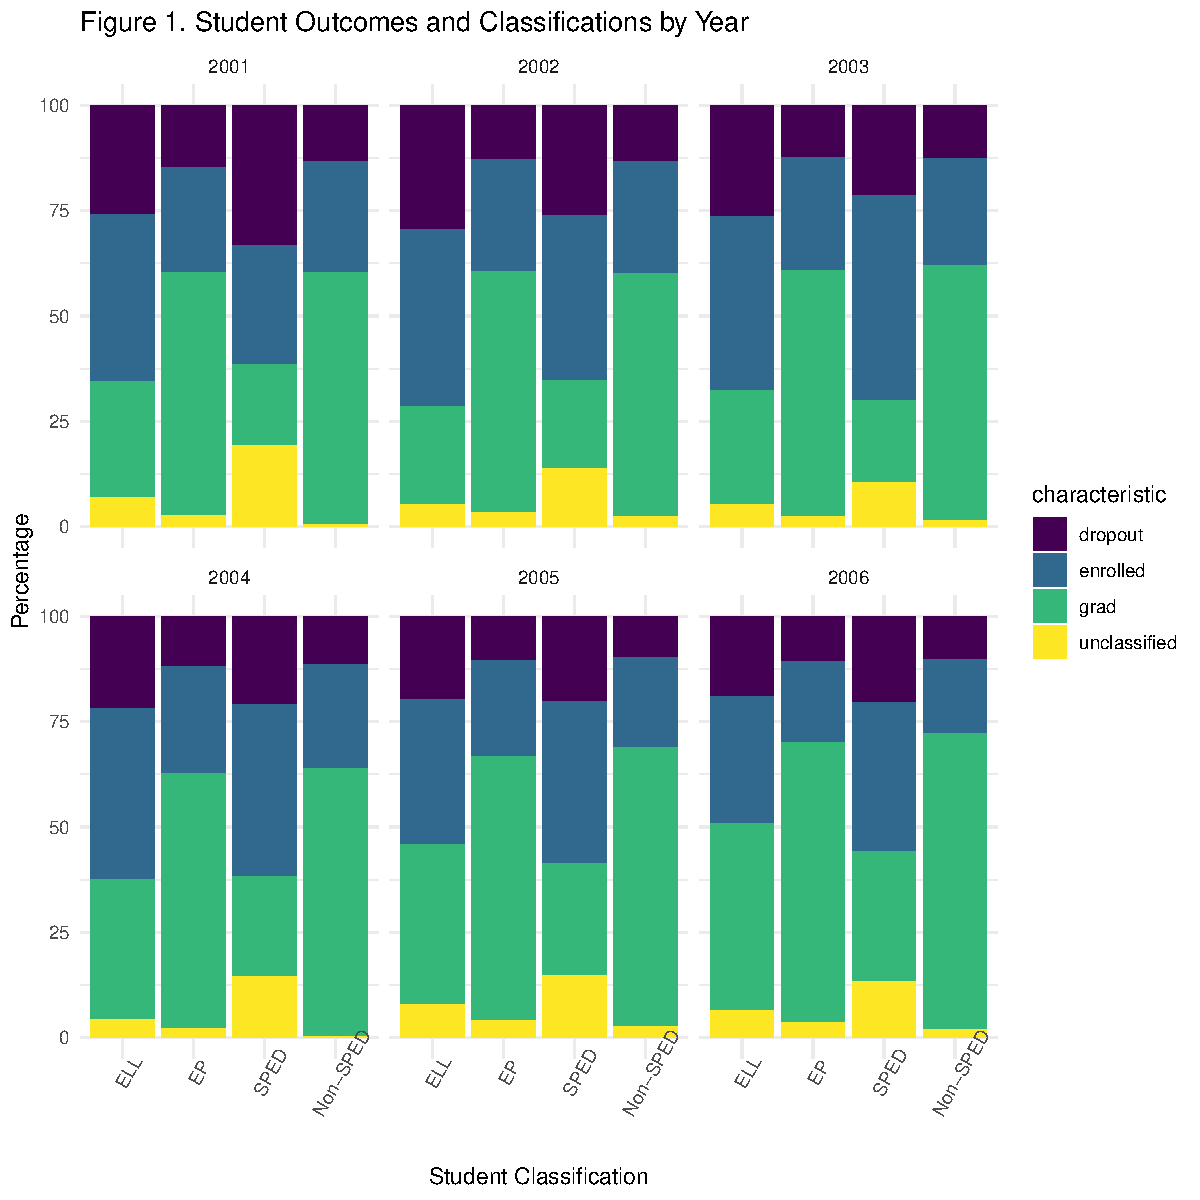
\includegraphics{EDLD_651_Final_Project_Draft_files/figure-latex/descriptives_of_dataset-1.pdf}

\begin{Shaded}
\begin{Highlighting}[]
\CommentTok{# We can also look at the following to get a general sense of the data:}
\CommentTok{# - total cohorts/grads, facet_wrap by borough}
\CommentTok{# - grad percentage by student_characteristic, then can do a deeper dive by borough}
\CommentTok{# - the above two repeated with dropout rate}
\end{Highlighting}
\end{Shaded}

\hypertarget{data-analysis}{%
\subsection{Data analysis}\label{data-analysis}}

All analysis were conducted in R, with heavy reliance upon the \texttt{\{tidyverse\}} packages to manipulate and visualize the data.

\hypertarget{results}{%
\section{Results}\label{results}}

\begin{Shaded}
\begin{Highlighting}[]
\CommentTok{#report graduation by borough}
\CommentTok{#report graduation by english language status}
\CommentTok{#report graduation by SPED status}
\CommentTok{#report graduation by borough & SPED status}
\CommentTok{#report graduation by borough & english learner status}
\end{Highlighting}
\end{Shaded}

\begin{Shaded}
\begin{Highlighting}[]
\NormalTok{new_grad }\OperatorTok\StringTok{ }
\StringTok{  }\KeywordTok{filter}\NormalTok{(student_characteristic }\OperatorTok{==}\StringTok{ "ELL"} \OperatorTok{|}\StringTok{ }
\StringTok{           }\NormalTok{student_characteristic }\OperatorTok{==}\StringTok{ "EP"}\NormalTok{) }\OperatorTok\StringTok{ }
\StringTok{  }\KeywordTok{mutate}\NormalTok{(}\DataTypeTok{Cohort =} \KeywordTok{factor}\NormalTok{(cohort)) }\OperatorTok\StringTok{ }
\StringTok{  }\KeywordTok{group_by}\NormalTok{(student_characteristic, borough) }\OperatorTok\StringTok{ }
\StringTok{  }\KeywordTok{ggplot}\NormalTok{(}\KeywordTok{aes}\NormalTok{(}\DataTypeTok{x =}\NormalTok{ student_characteristic, }
             \DataTypeTok{y =}\NormalTok{ total_grads_percent_of_cohort)) }\OperatorTok{+}
\StringTok{  }\KeywordTok{geom_jitter}\NormalTok{(}\KeywordTok{aes}\NormalTok{(}\DataTypeTok{color =}\NormalTok{ Cohort)) }\OperatorTok{+}\StringTok{ }\KeywordTok{facet_wrap}\NormalTok{(}\OperatorTok{~}\NormalTok{borough) }\OperatorTok{+}\StringTok{ }
\StringTok{  }\KeywordTok{labs}\NormalTok{(}\DataTypeTok{title =} \StringTok{'Figure 1. Graduation Rates in NYC by English Learner Status'}\NormalTok{,}
       \DataTypeTok{subtitle =} \StringTok{'Boroughs are reported separetely with lighter dots indicating more recent years'}\NormalTok{,}
       \DataTypeTok{y =} \StringTok{'Percent of total cohort'}\NormalTok{,}
       \DataTypeTok{x =} \StringTok{'Student Characteristic'}\NormalTok{)}
\end{Highlighting}
\end{Shaded}

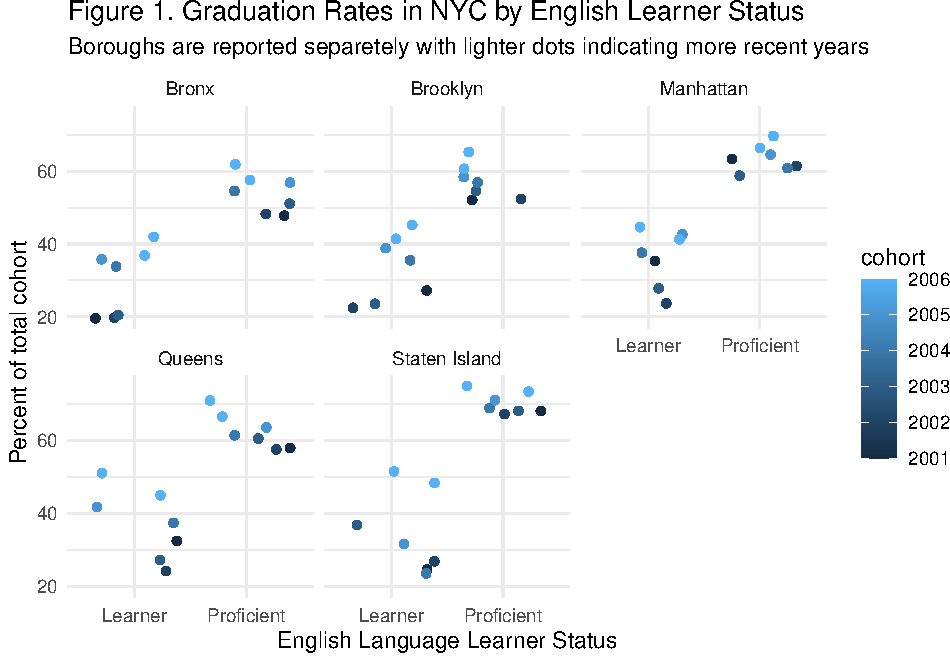
\includegraphics{EDLD_651_Final_Project_Draft_files/figure-latex/graph_results-1.pdf}

\begin{Shaded}
\begin{Highlighting}[]
\NormalTok{new_grad }\OperatorTok\StringTok{ }
\StringTok{  }\KeywordTok{filter}\NormalTok{(student_characteristic }\OperatorTok{==}\StringTok{ "SPED"} \OperatorTok{|}\StringTok{ }
\StringTok{           }\NormalTok{student_characteristic }\OperatorTok{==}\StringTok{ "Non-SPED"}\NormalTok{) }\OperatorTok\StringTok{ }
\StringTok{  }\KeywordTok{mutate}\NormalTok{(}\DataTypeTok{Cohort =} \KeywordTok{factor}\NormalTok{(cohort)) }\OperatorTok\StringTok{ }
\StringTok{  }\KeywordTok{group_by}\NormalTok{(student_characteristic, borough) }\OperatorTok\StringTok{ }
\StringTok{  }\KeywordTok{ggplot}\NormalTok{(}\KeywordTok{aes}\NormalTok{(}\DataTypeTok{x =}\NormalTok{ student_characteristic, }
             \DataTypeTok{y =}\NormalTok{ total_grads_percent_of_cohort)) }\OperatorTok{+}
\StringTok{  }\KeywordTok{geom_jitter}\NormalTok{(}\KeywordTok{aes}\NormalTok{(}\DataTypeTok{color =}\NormalTok{ Cohort)) }\OperatorTok{+}\StringTok{ }
\StringTok{  }\KeywordTok{facet_wrap}\NormalTok{(}\OperatorTok{~}\NormalTok{borough) }\OperatorTok{+}\StringTok{ }
\StringTok{  }\KeywordTok{labs}\NormalTok{(}\DataTypeTok{title =} \StringTok{'Figure 1. Graduation Rates in NYC by English Learner Status'}\NormalTok{,}
       \DataTypeTok{subtitle =} \StringTok{'Boroughs are reported separetely with lighter dots indicating more recent years'}\NormalTok{,}
       \DataTypeTok{y =} \StringTok{'Percent of total cohort'}\NormalTok{,}
       \DataTypeTok{x =} \StringTok{'Student Characteristic'}\NormalTok{)}
\end{Highlighting}
\end{Shaded}

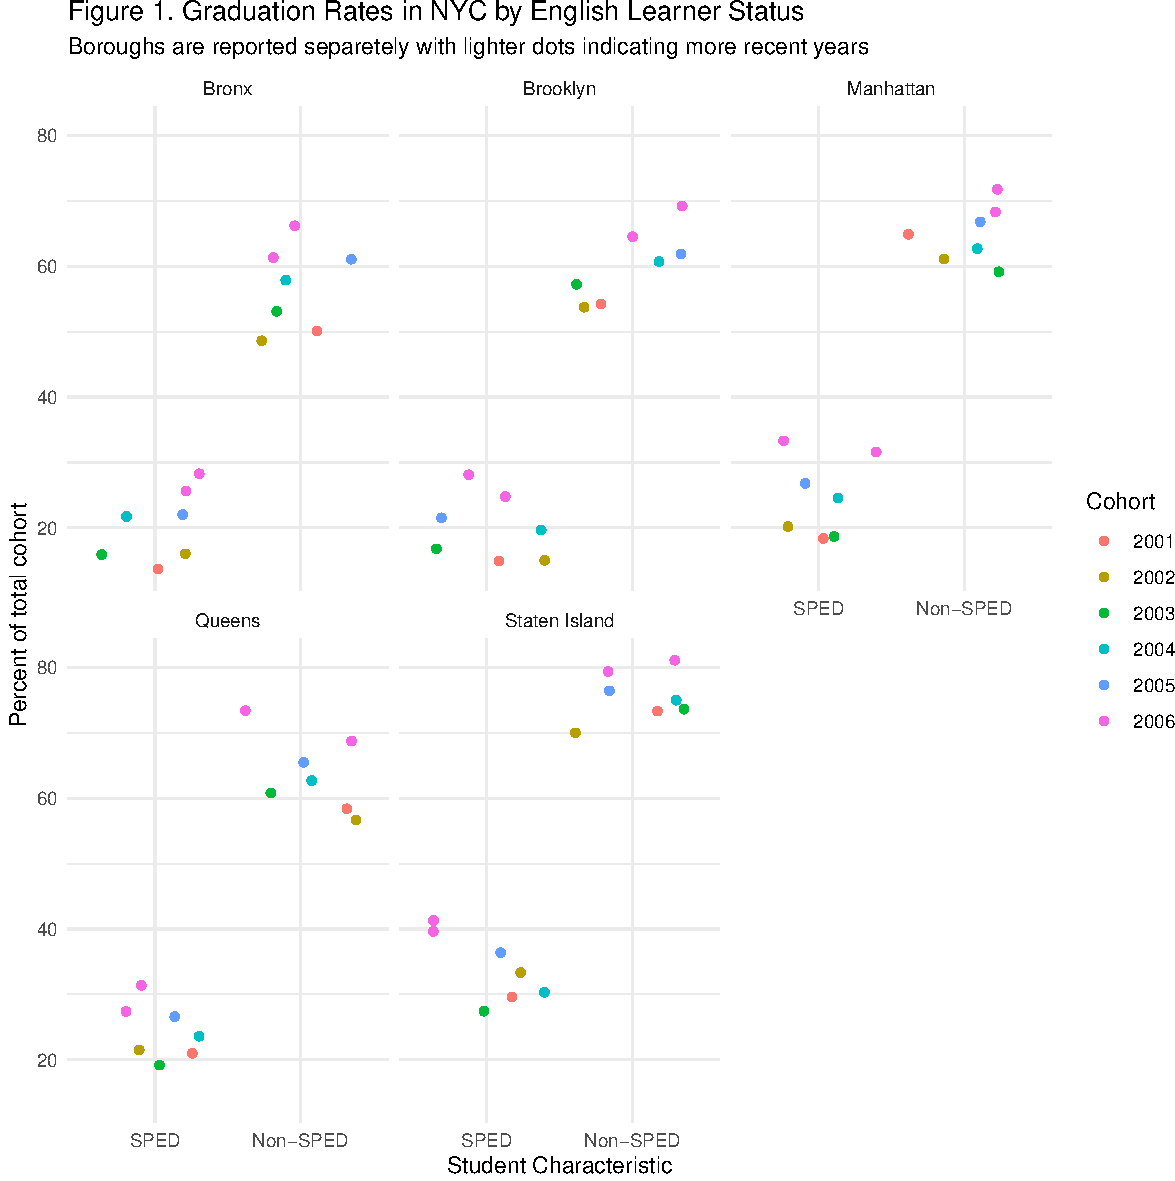
\includegraphics{EDLD_651_Final_Project_Draft_files/figure-latex/graph_results2-1.pdf}

\hypertarget{discussion}{%
\section{Discussion}\label{discussion}}

Differences appear to be blah by blah for blah. XYZ boroughs should consider blah blah blah, based on the results. Inferential tests are recommended for next directions.

\newpage

\hypertarget{references}{%
\section{References}\label{references}}

\begingroup
\setlength{\parindent}{-0.5in}
\setlength{\leftskip}{0.5in}

\hypertarget{refs}{}

\endgroup


\end{document}
